\chapter{Signal Extraction\label{ch:signalextraction}}

After applying the preselection, event classification, and mass windows, the signal efficiency
and event yields are examined, as discussed in Section~\ref{sec:yields}. Then fits are performed
to the signal simulation for estimating the expected signal shape and to the data for estimating
the expected background shape. The fits are discussed in Sections~\ref{sec:resfits} and
\ref{sec:nonresfits} for the resonant and nonresonant searches, respectively.

\section{Signal Efficiencies and Yields\label{sec:yields}}

The signal efficiency as a function of $m_X$ for the resonant search is summarized in
Figure~\ref{fig:eff_res}. The signal efficiency increases from 260 GeV to 900 GeV
due to improved photon and jet reconstruction. The signal efficiency
peaks and then drops at 900 GeV due to the merging of the jets from the decay $\Hbb$ into
a single jet. For future consideration in extending the search above 1.1 TeV,
jet substructure techniques would be necessary to resolve the merging of the two
jets~\cite{Ellis:2009su}.
Both categories contribute approximately equally to the overall efficiency.

\begin{figure}[htbp!]
 \begin{center}
    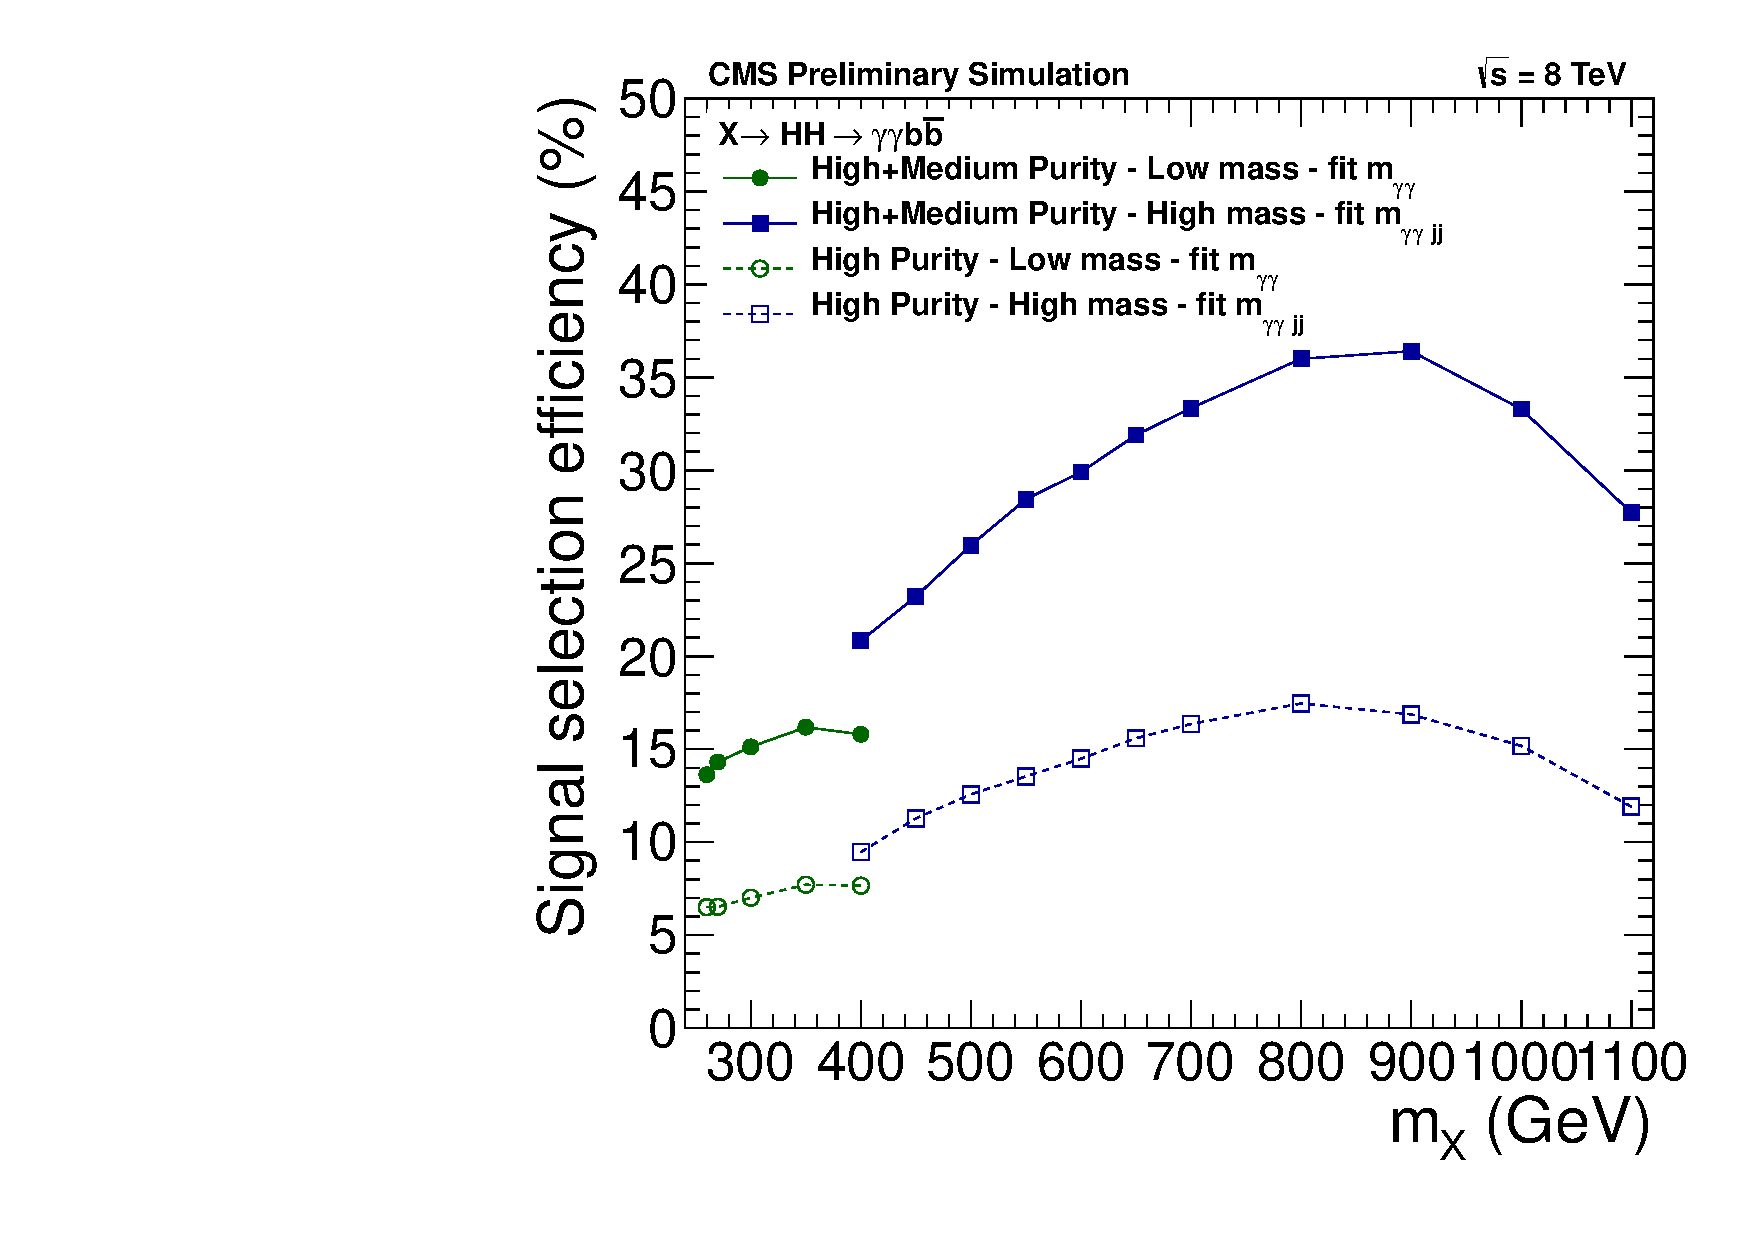
\includegraphics[width=0.60\textwidth]{figures/results/eff_all.pdf}
      \end{center}
\caption{Signal efficiency for the resonant search for the final selection.}
\label{fig:eff_res}
\end{figure}

The relative yields for the nonresonant backgrounds in the low-mass resonant search at $m_X = 300$~GeV
are summarized in
Table~\ref{table:yield_lowmass_res}. There is a normalization disagreement in the
$\gamma\gamma j$ and $\gamma j$ contributions as the simulation has limitations in modeling
QCD with one or two hard photons. As a result, the relative yields as a percentage of the total estimated
nonresonant background are given.
The relavitve yields for the nonresonant backgrounds in the high-mass resonant search are summarized in
Table~\ref{table:yield_highmass_res}. For this search, the requirements are independent of
the mass hypothesis, and again the relative yields as a percentage of the total estimated nonresonant
background are given.

\begin{table}[htbp!]
  \centering
  \renewcommand{\arraystretch}{1.4}
  \caption{Relative event yields for the nonresonant backgrounds in the low-mass resonant search
at 300 GeV. Note that there is a normalization disagreement coming from the shortcomings of
simulating QCD with one or two hard photons, so percentages are given instead of numbers
of events.}
  \begin{tabular}{|c|c|c|}
\hline
Sample & High purity & Medium purity\\
\hline
Radion (300$~$GeV, $\Lambda_R$=1TeV)  & 18.73 & 21.66     \\
\hline
ggF $\Hgg$                &  0.02  &  0.19 \\
VBF $\Hgg$                &  0.00  &  0.04 \\
$WH(\gamma\gamma)$        &  0.00  &  0.05 \\
$ZH(\gamma\gamma)$        &  0.00  &  0.03 \\
$t\bar{t}H(\gamma\gamma)$ &  0.10  &  0.15 \\
\hline
$\gamma\gamma j$                      & 8.9  &  188  \\
$\gamma j$                            & 0.00 &  9.2  \\ 
QCD                                   & 0.00 &  0.00 \\ 
$Z/\gamma^*\rightarrow\ell^+\ell^- + Z(\ell^+\ell^-)\gamma + W(\ell\nu)\gamma\gamma$ & 0.00 &  0.21 \\
$t\bar{t}\gamma\gamma + t\gamma\gamma + t\bar{t}\gamma j$ & 0.44 &  1.2  \\
\hline
Data                                  & 21 & 230 \\
\hline
\end{tabular}

  \label{table:yield_lowmass_res}
\end{table}

\begin{table}[htbp!]
  \centering
  \renewcommand{\arraystretch}{1.4}
  \caption{Relative event yields for the nonresonant backgrounds in the high-mass resonant search.
Note that there is a normalization disagreement coming from the shortcomings of simulating QCD with one
or two hard photons, so percentages are given instead of numbers of events.}
  \begin{tabular}{|c|c|c|}
\hline
Sample & High purity & Medium purity\\
\hline
Radion (500$~$GeV, $\Lambda_R$=1TeV)        &  6.08  & 6.47     \\
Radion (700$~$GeV, $\Lambda_R$=1TeV)        &  2.92  & 3.03     \\
Radion (1000$~$GeV, $\Lambda_R$=1TeV)       &  0.94  & 1.12     \\
\hline
ggF $\Hgg$                &  0.07  &  0.6  \\
VBF $\Hgg$                &  0.01  &  0.12 \\
$WH(\gamma\gamma)$        &  0.00  &  0.10 \\
$ZH(\gamma\gamma)$        &  0.03  &  0.07 \\
$t\bar{t}H(\gamma\gamma)$ &  0.24  &  0.50 \\
\hline
$\gamma\gamma j$                      & 3.0  &  70   \\
$\gamma j$                            & 0.00 &  3.0  \\
QCD                                   & 0.00 &  0.00 \\
& 8.9  &  188  \\
& 0.00 &  9.2  \\ 
& 0.00 &  0.00 \\ 
$Z/\gamma^*\rightarrow\ell^+\ell^- + Z(\ell^+\ell^-)\gamma + W(\ell\nu)\gamma\gamma$ & 0.00 &  0.08 \\
$t\bar{t}\gamma\gamma + t\gamma\gamma + t\bar{t}\gamma j$ & 0.15 &  0.55 \\
\hline
Data                                  & 8 & 79 \\
\hline
\end{tabular}

  \label{table:yield_highmass_res}
\end{table}

The relavive yields for the nonresonant backgrounds in the nonresonant search are summarized in
Table~\ref{table:yield_nonres}. The yields are greater in the nonresonant search
because the $\Mggjjk$ spectrum is less
discriminating than in the low-mass resonant search and because the $\Mjj$ spectrum is
fit on the range $\Mjj \in [60,180]$~GeV rather than selected on a narrower range.
The yields for the SM nonresonant signal and resonant backgrounds as well as the counts for
data are shown in Table~\ref{table:yield_data_nonres}.

\begin{table}[htbp!]
  \centering
  \renewcommand{\arraystretch}{1.4}
  \caption{Event yields for the nonresonant search. Expectations are given for
the SM nonresonant signal, resonant background, and nonresonant background.
Counts are given for data. Note that
there is a normalization disagreement coming from the shortcomings of simulating QCD with one
or two hard photons.}
  \begin{tabular}{|c|c|c|c|c|}
\hline
 & \multicolumn{2}{c|}{High Purity} & \multicolumn{2}{c|}{Medium Purity} \\
Sample & high $\Mggjjk$ & low $\Mggjjk$ & high $\Mggjjk$ & low $\Mggjjk$ \\
\hline
SM nonresonant $HH$ & 2.03 & 0.28 & 1.99 & 0.20\\
%SM: $\kapl = 1$, $\kapt = 1$, $\ctwo = 0$ & 2.03 & 0.28 & 1.99 & 0.20\\
%$\kapl = 20$, $\kapt = 1$, $\ctwo = 0$ & 78.7 & 102 & 86.5 & 96.5\\
%$\kapl = 1$, $\kapt = 1$, $\ctwo = -2$  & 103 & 16.2 & 101 & 16.5\\
%lam=1  yt=1 c2=0  xsec = 9.96
%lam=20 yt=1 c2=0  xsec = 1046
%lam=1  yt=1 c2=-2 xsec  = 511
\hline
ggF $\Hgg$                &  0.05 & 0.04 & 0.29 & 0.32\\
VBF $\Hgg$                &  0.01 & 0.01 & 0.05 & 0.05\\
$WH(\gamma\gamma)$        &  0.00 & 0.00 & 0.12 & 0.09\\     
$ZH(\gamma\gamma)$        &  0.04 & 0.02 & 0.07 & 0.05\\
$t\bar{t}H(\gamma\gamma)$ &  0.16 & 0.17 & 0.30 & 0.17\\
$b\bar{b}H(\gamma\gamma)$ &  0.00 & 0.01 & 0.01 & 0.04\\  
\hline
$\gamma\gamma j$     &  13 & 21  & 151 & 268 \\
$\gamma j$           & 0.00& 4.3 & 28  & 53  \\
QCD                  & 0.00& 0.00& 0.00& 0.00\\
$Z/\gamma^*\rightarrow\ell^+\ell^- + Z(\ell^+\ell^-)\gamma + W(\ell\nu)\gamma\gamma$
   & 0.00 & 0.01 & 2.3 & 0.18 \\
$t\bar{t}\gamma\gamma + t\gamma\gamma + t\bar{t}\gamma j$ &  1.3 & 2.2 & 3.3 & 3.4 \\
\hline
Data                                  & 41 & 136 & 37 & 319 \\
\hline
\end{tabular}

  \label{table:yield_nonres}
\end{table}

\begin{table}[htbp!]
  \centering
  \renewcommand{\arraystretch}{1.4}
  \caption{Event yields for the nonresonant search. Expectations are given for
the SM nonresonant signal and resonant backgrounds. Counts are given for data.}
  \begin{tabular}{|c|c|c|c|c|}
\hline
 & \multicolumn{2}{c|}{High Purity} & \multicolumn{2}{c|}{Medium Purity} \\
Sample & high $\Mggjjk$ & low $\Mggjjk$ & high $\Mggjjk$ & low $\Mggjjk$ \\
\hline
SM nonresonant $HH$ & 2.03 & 0.28 & 1.99 & 0.20\\
%SM: $\kapl = 1$, $\kapt = 1$, $\ctwo = 0$ & 2.03 & 0.28 & 1.99 & 0.20\\
%$\kapl = 20$, $\kapt = 1$, $\ctwo = 0$ & 78.7 & 102 & 86.5 & 96.5\\
%$\kapl = 1$, $\kapt = 1$, $\ctwo = -2$  & 103 & 16.2 & 101 & 16.5\\
%lam=1  yt=1 c2=0  xsec = 9.96
%lam=20 yt=1 c2=0  xsec = 1046
%lam=1  yt=1 c2=-2 xsec  = 511
\hline
ggF $\Hgg$                &  0.05 & 0.04 & 0.29 & 0.32\\
VBF $\Hgg$                &  0.01 & 0.01 & 0.05 & 0.05\\
$WH(\gamma\gamma)$      &$<$~0.01&$<$~0.01&0.12 & 0.09\\     
$ZH(\gamma\gamma)$        &  0.04 & 0.02 & 0.07 & 0.05\\
$t\bar{t}H(\gamma\gamma)$ &  0.16 & 0.17 & 0.30 & 0.17\\
$b\bar{b}H(\gamma\gamma)$ &$<$~0.01&0.01 & 0.01 & 0.04\\  
\hline
Data                                  & 41 & 136 & 37 & 319 \\
\hline
\end{tabular}

  \label{table:yield_data_nonres}
\end{table}

\section{Resonant Fits\label{sec:resfits}}

\subsection{Low-mass Resonant Fits\label{subsec:resfits_lowmass}}

For the low-mass resonant search, the signal yield is extracted by fitting the $\Mgg$ spectrum.
The signal model is built for each mass hypothesis by fitting the $\Mgg$ spectrum
in the simulation sample
separately for the two categories. The functional form used is the sum of a Crystal Ball and
a Gaussian, with constrained to have the same mean,
where the former models the core of the distribution and the latter models the
tails. The position of the peak and the spread are independent of the resonant mass and the
category. Figure~\ref{fig:sigfit_300} shows an example of the signal fit for a mass hypothesis of
300 GeV.

\begin{figure}[htbp!]
 \begin{center}
   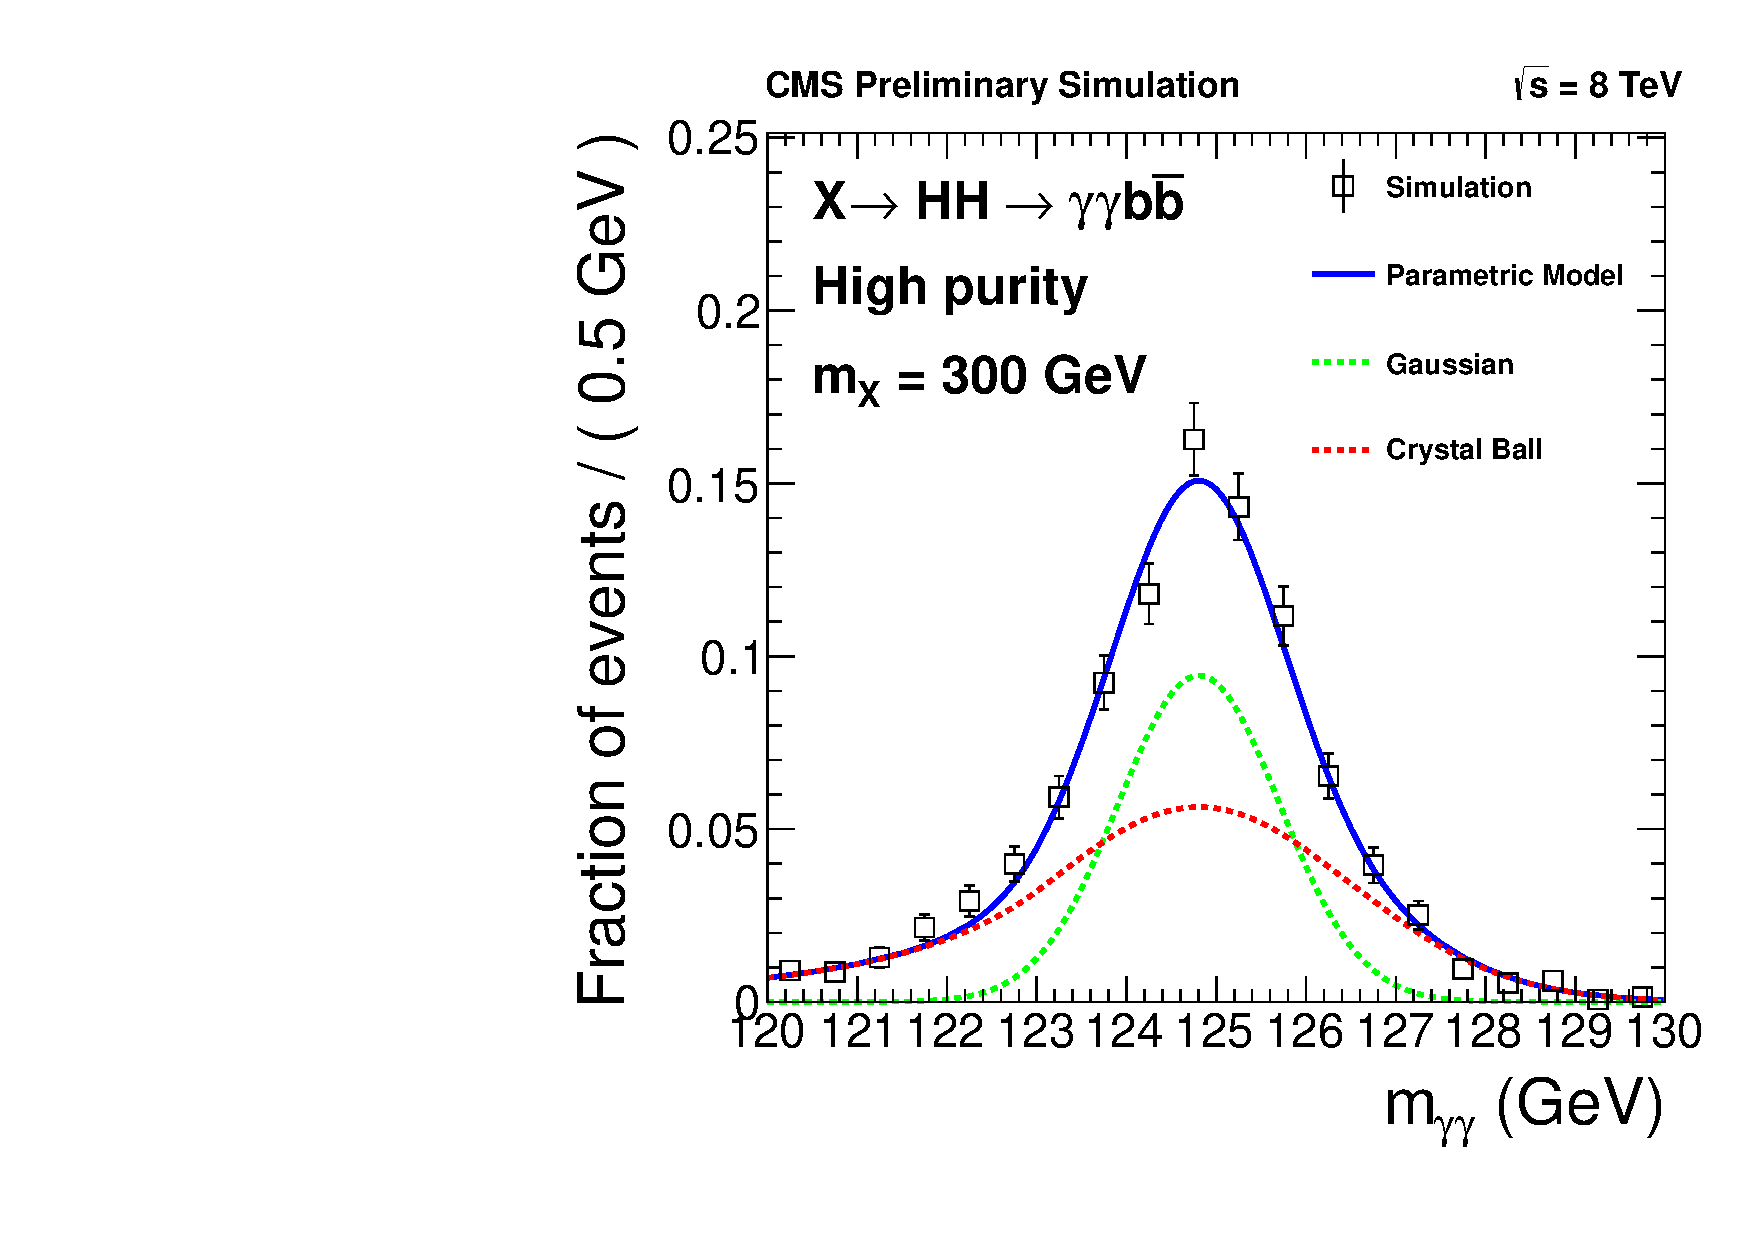
\includegraphics[width=0.45\textwidth]{figures/results/sigmodel_cat0_300.pdf}
   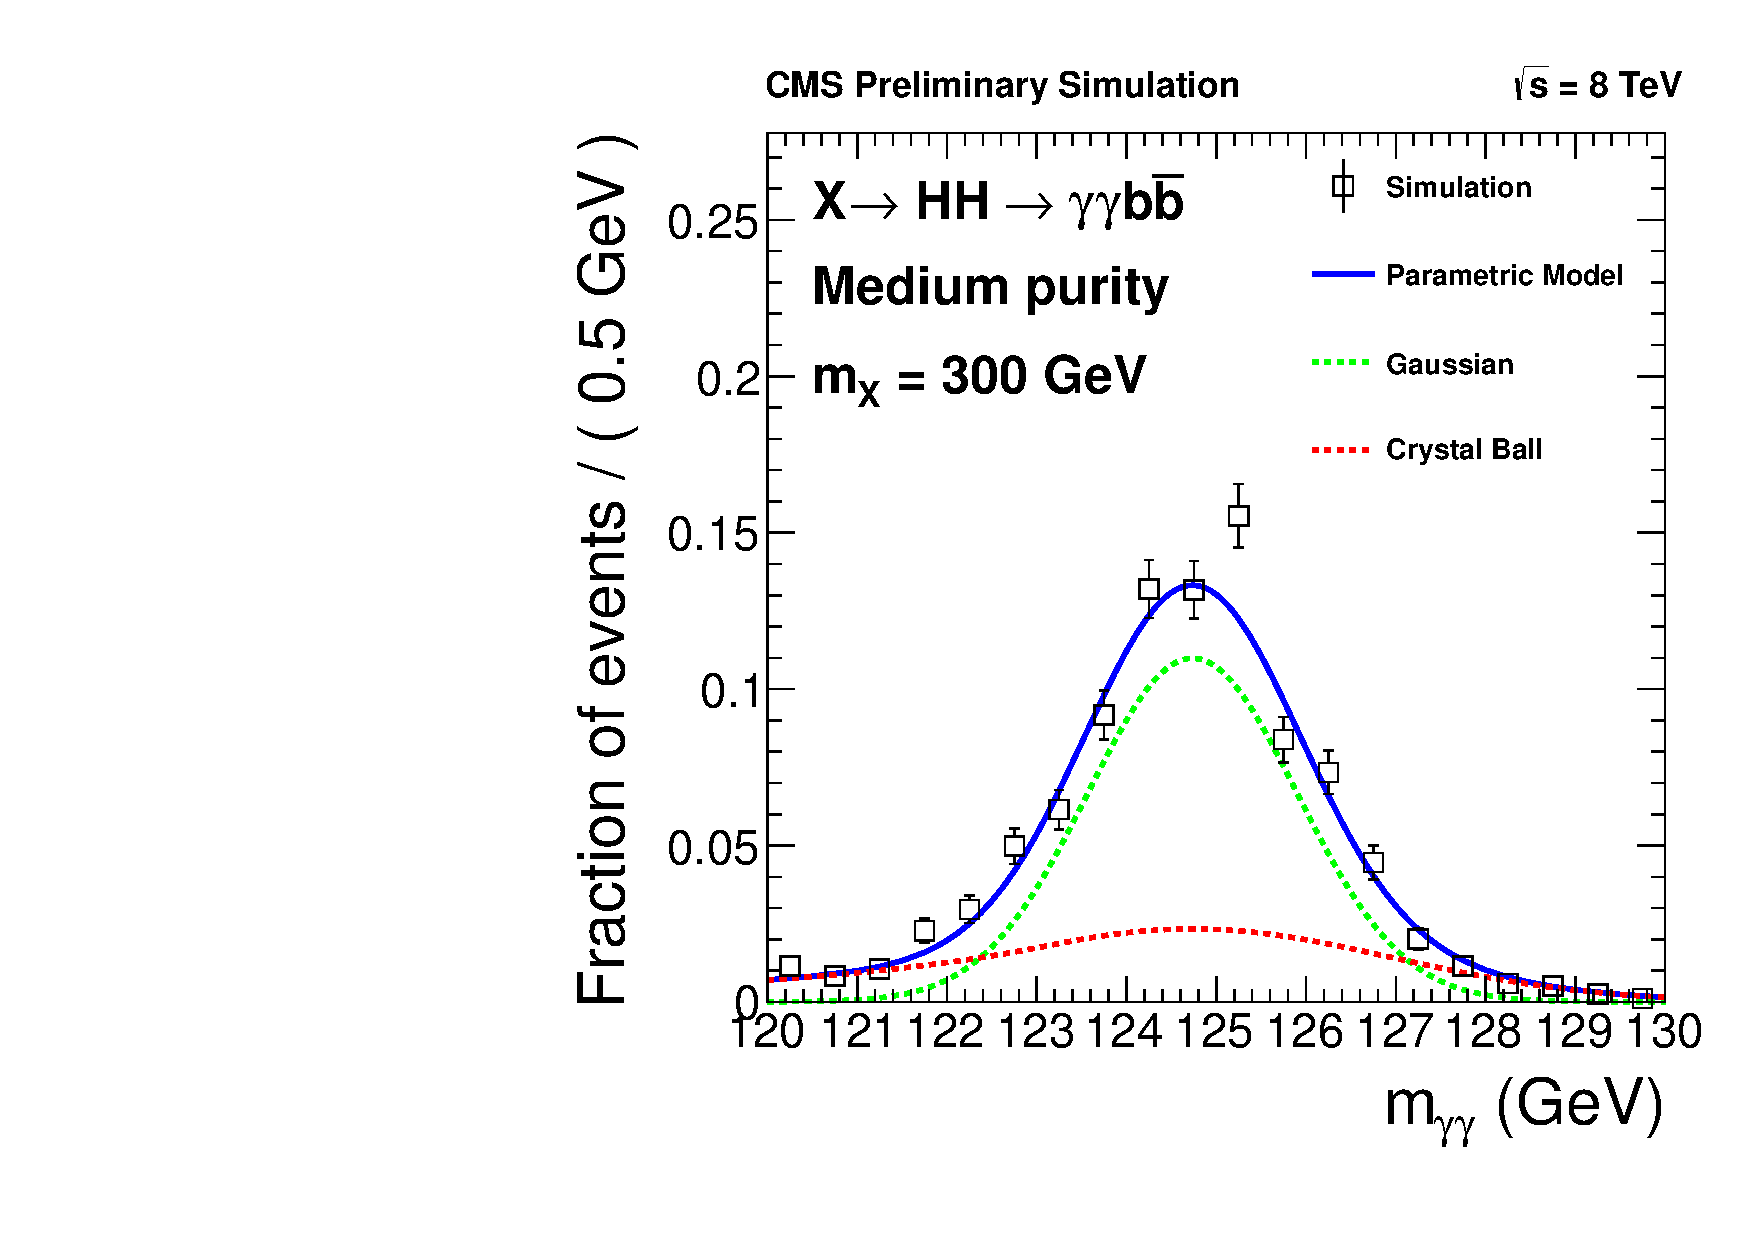
\includegraphics[width=0.45\textwidth]{figures/results/sigmodel_cat1_300.pdf}
 \end{center}
\caption{Simulated signal shape in the $\Mgg$ spectrum for the high-purity (left) and medium-purity
(right) categories for the Radion with mass 300 GeV. The open squares and corresponding
statistical uncertainties represent the simulation.
The blue line represents the signal model fitted to the simulation, while the green dashed line
and the red dashed line represent the two components of the signal model.}
\label{fig:sigfit_300}
\end{figure}

The background estimation is performed by fitting the same distribution in data
for each category on the interval
$[100, 180]$~GeV. This procedure is completely data-driven, and as such it is important
to verify that the choice of the function does not bias the estimate of the signal
strength obtained from the fit to data with the sum of signal and background components.
The bias is estimated by considering a set of truth models which approximately describe the background.
For each truth model a large set of pseudo-data is generated and fitted by the sum of a candidate
background model and the signal model. The bias is defined as the ratio of the extracted signal strength
$\mu$ divided by the associated statistical uncertainty $\sigma_\mu$ and
is considered negligible if
\begin{equation}
\left|\text{median}\left(\frac{\mu}{\sigma_\mu}\right)\right| < 14\% \,.
\end{equation}
For both categories, more than one unbiased background candidate function is identified.
For the background fit,
a power law is chosen for both categories. Figures~\ref{fig:datafit_260} and \ref{fig:datafit_300}
shows the background fits to the data for four mass hypotheses.

\begin{figure}[htbp!]
 \begin{center}
   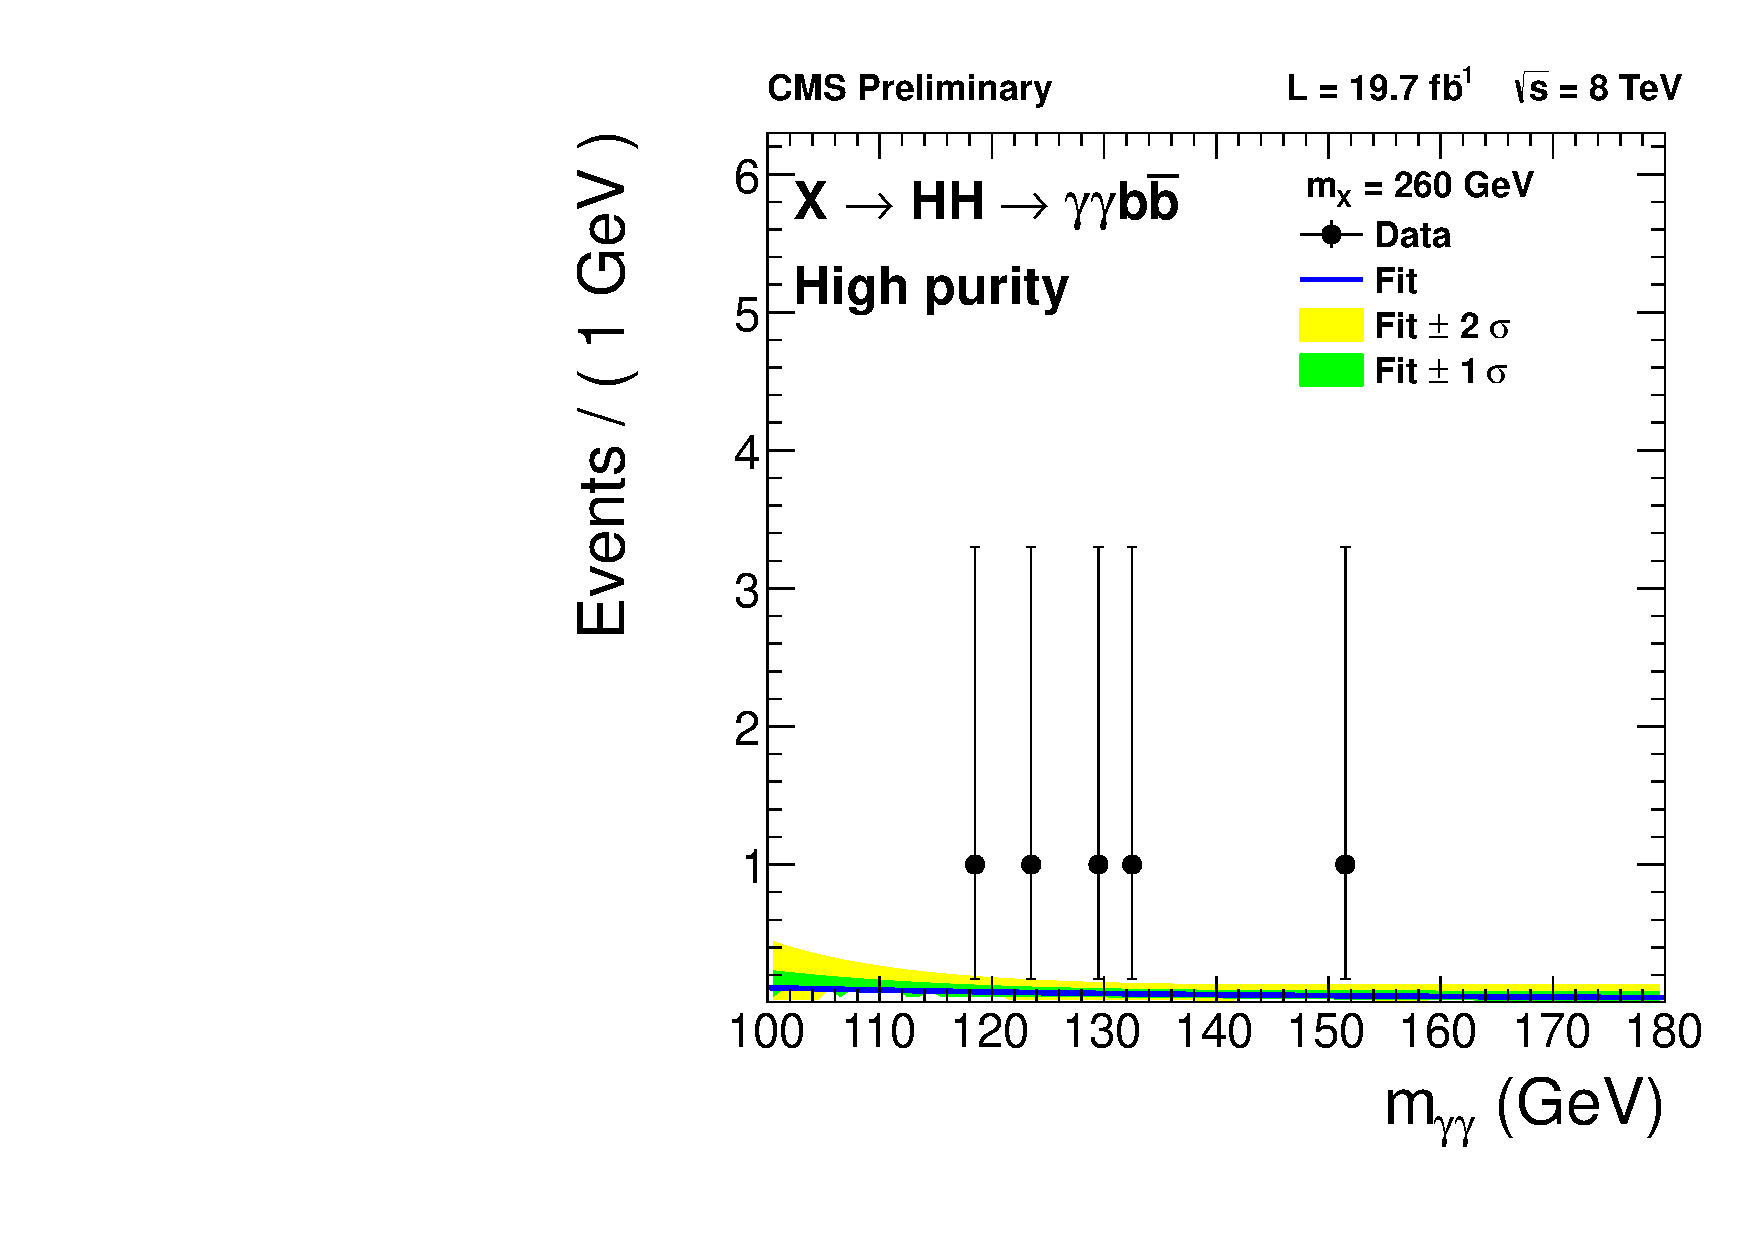
\includegraphics[width=0.45\textwidth]{figures/results/databkgoversig_cat0_260GeV.pdf}
   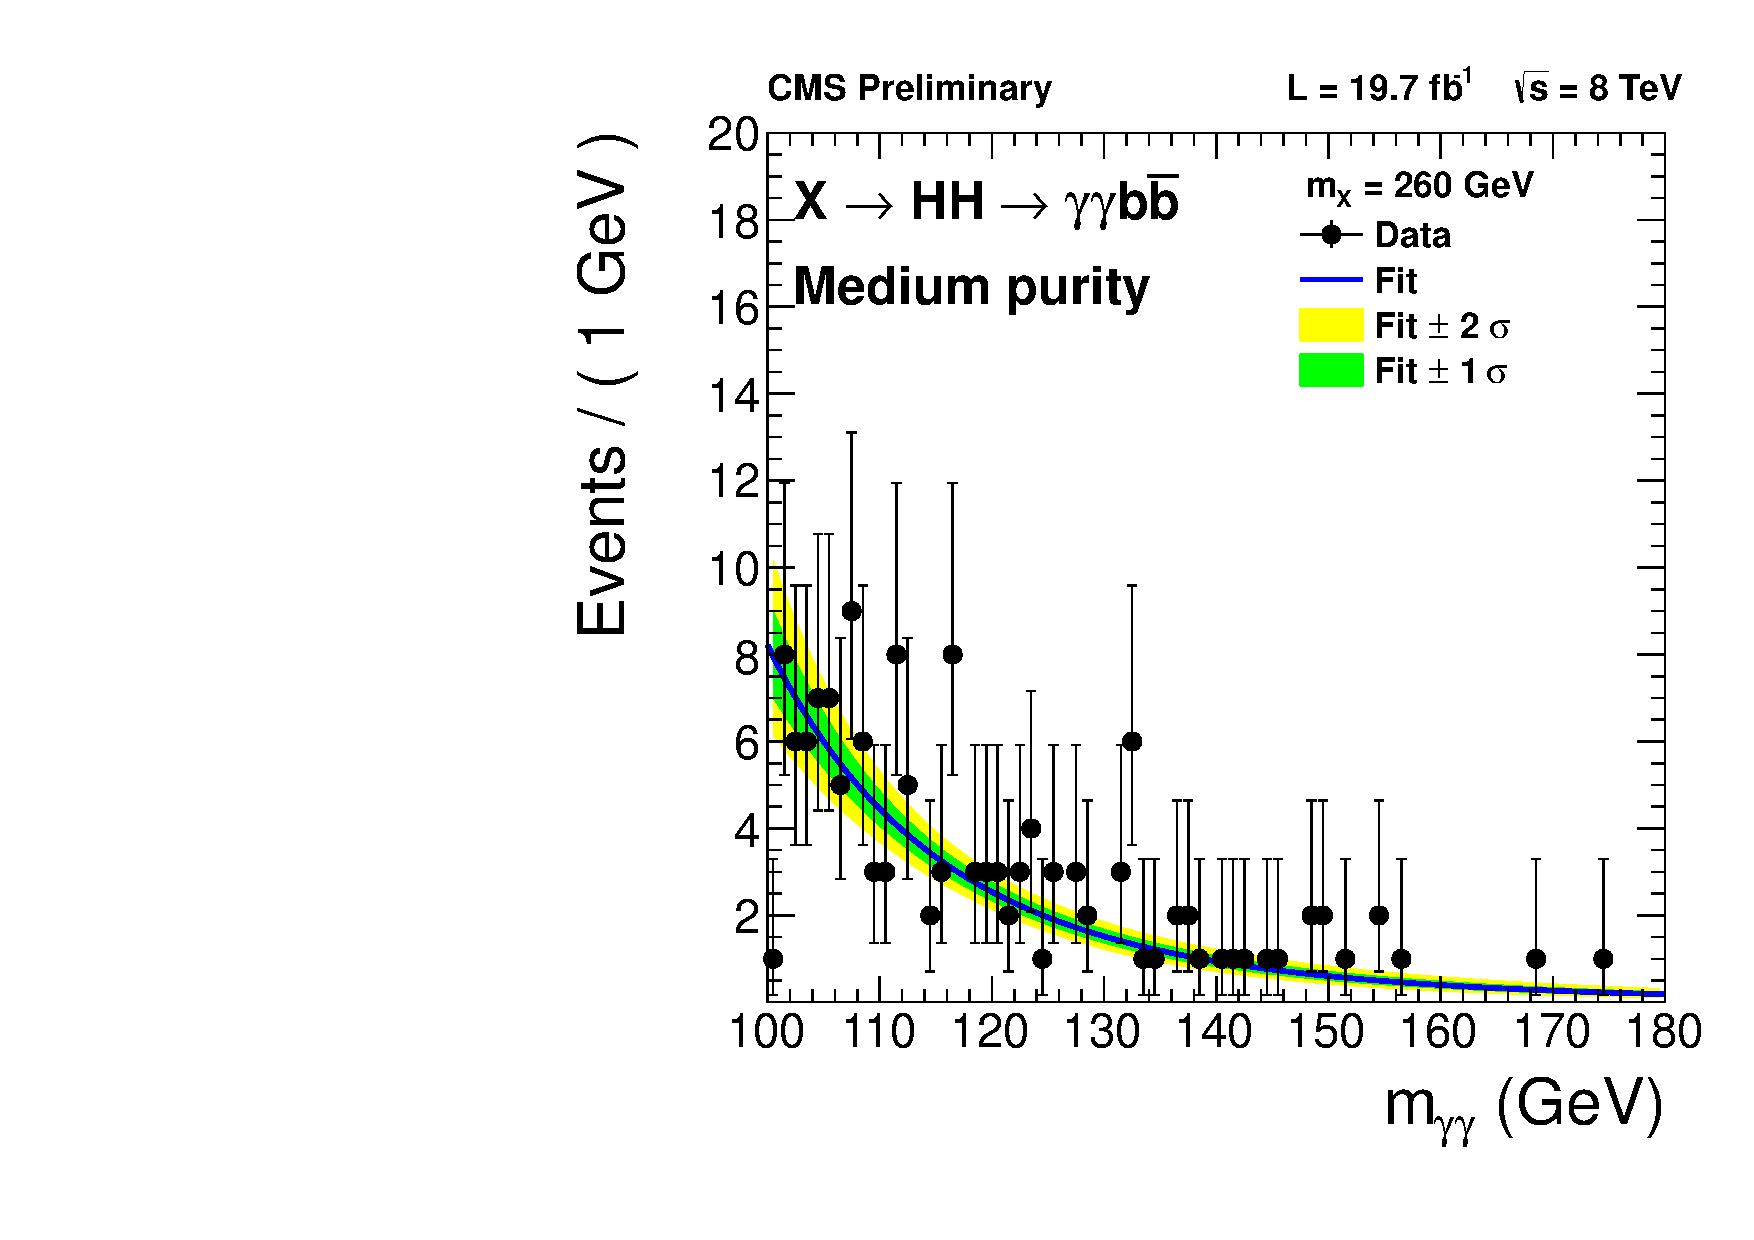
\includegraphics[width=0.45\textwidth]{figures/results/databkgoversig_cat1_260GeV.pdf}
   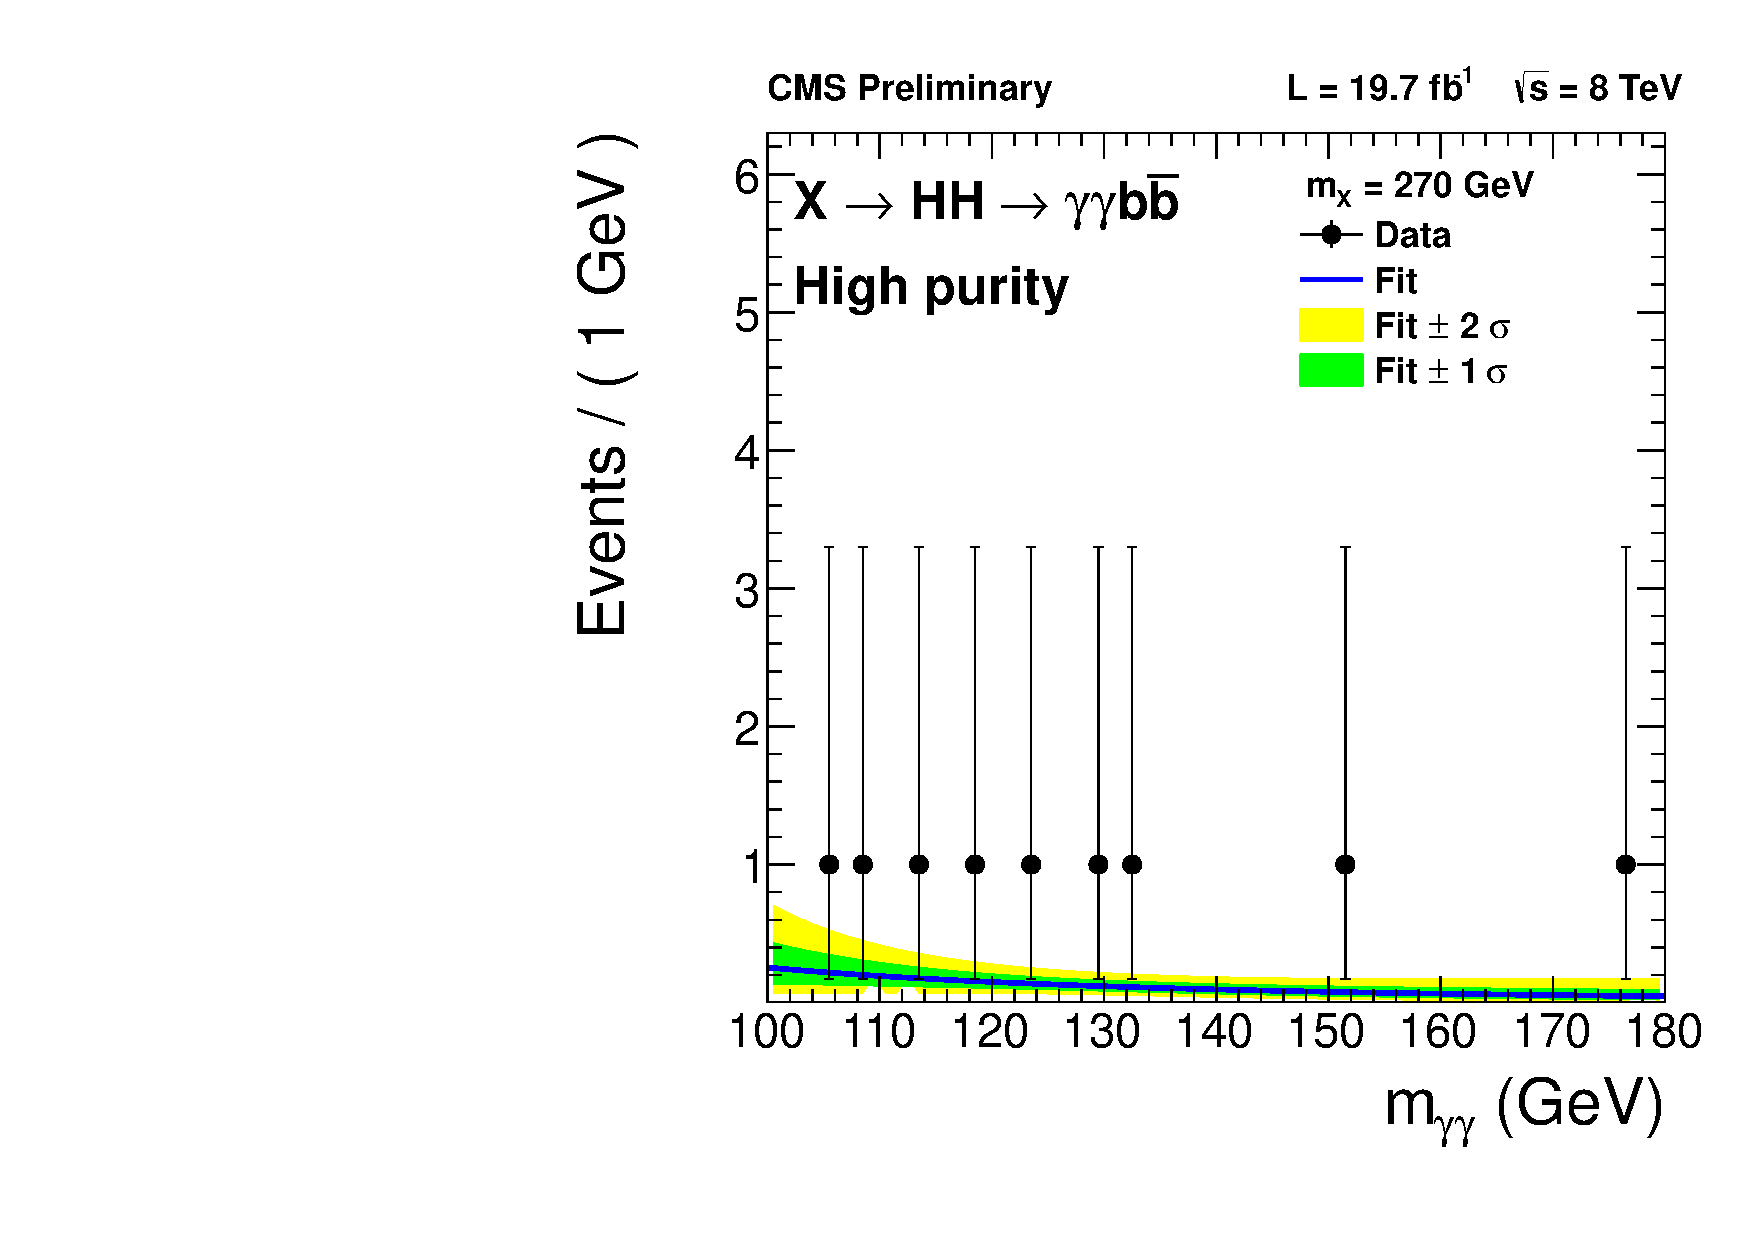
\includegraphics[width=0.45\textwidth]{figures/results/databkgoversig_cat0_270GeV.pdf}
   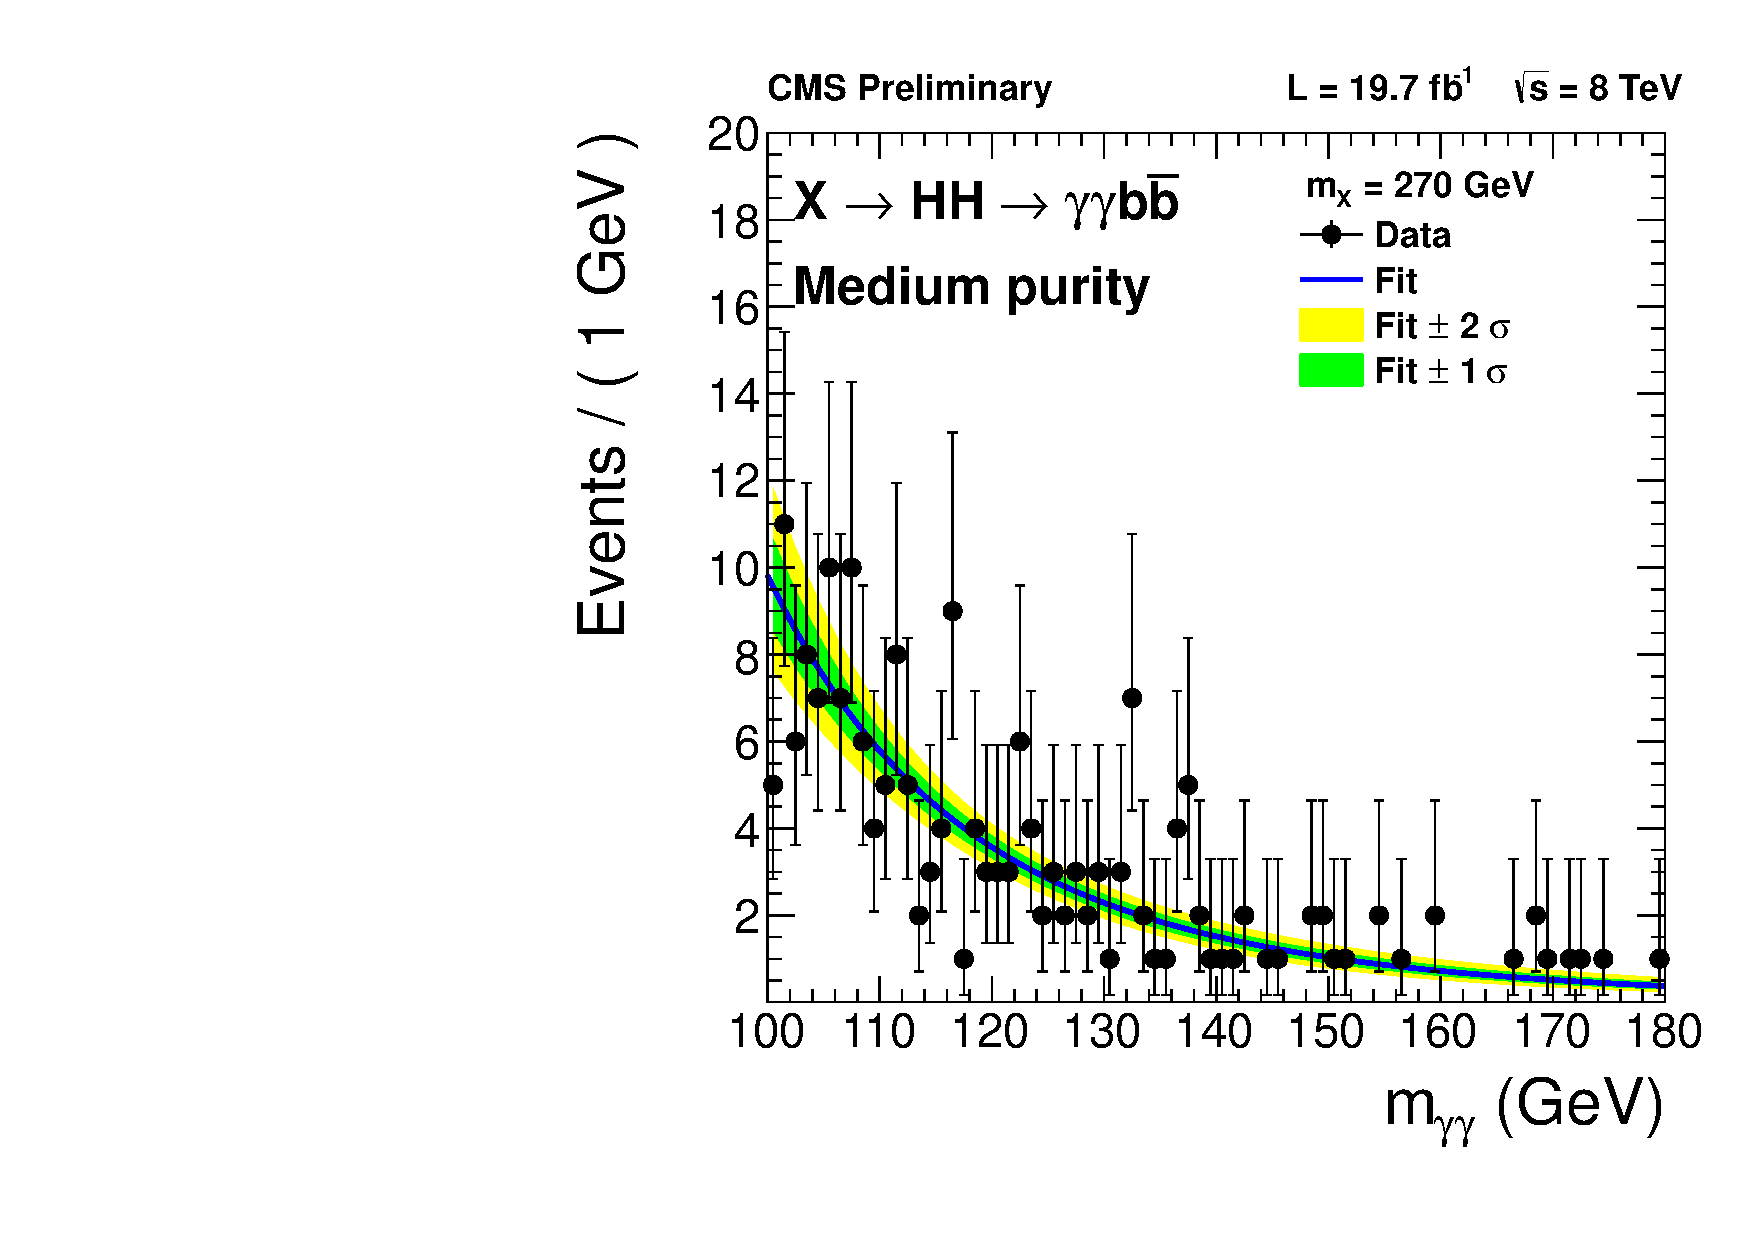
\includegraphics[width=0.45\textwidth]{figures/results/databkgoversig_cat1_270GeV.pdf}
 \end{center}
\caption{Events in the $\Mgg$ spectrum in the high-purity (left column) and medium-purity
(right column) categories for the resonance mass hypotheses 260 GeV (top row) and 270 GeV (bottom row).
The nonresonant component of the background fit is shown in blue
with its corresponding 1$\sigma$ and 2$\sigma$ confidence intervals.}
\label{fig:datafit_260}
\end{figure}

\begin{figure}[htbp!]
 \begin{center}
   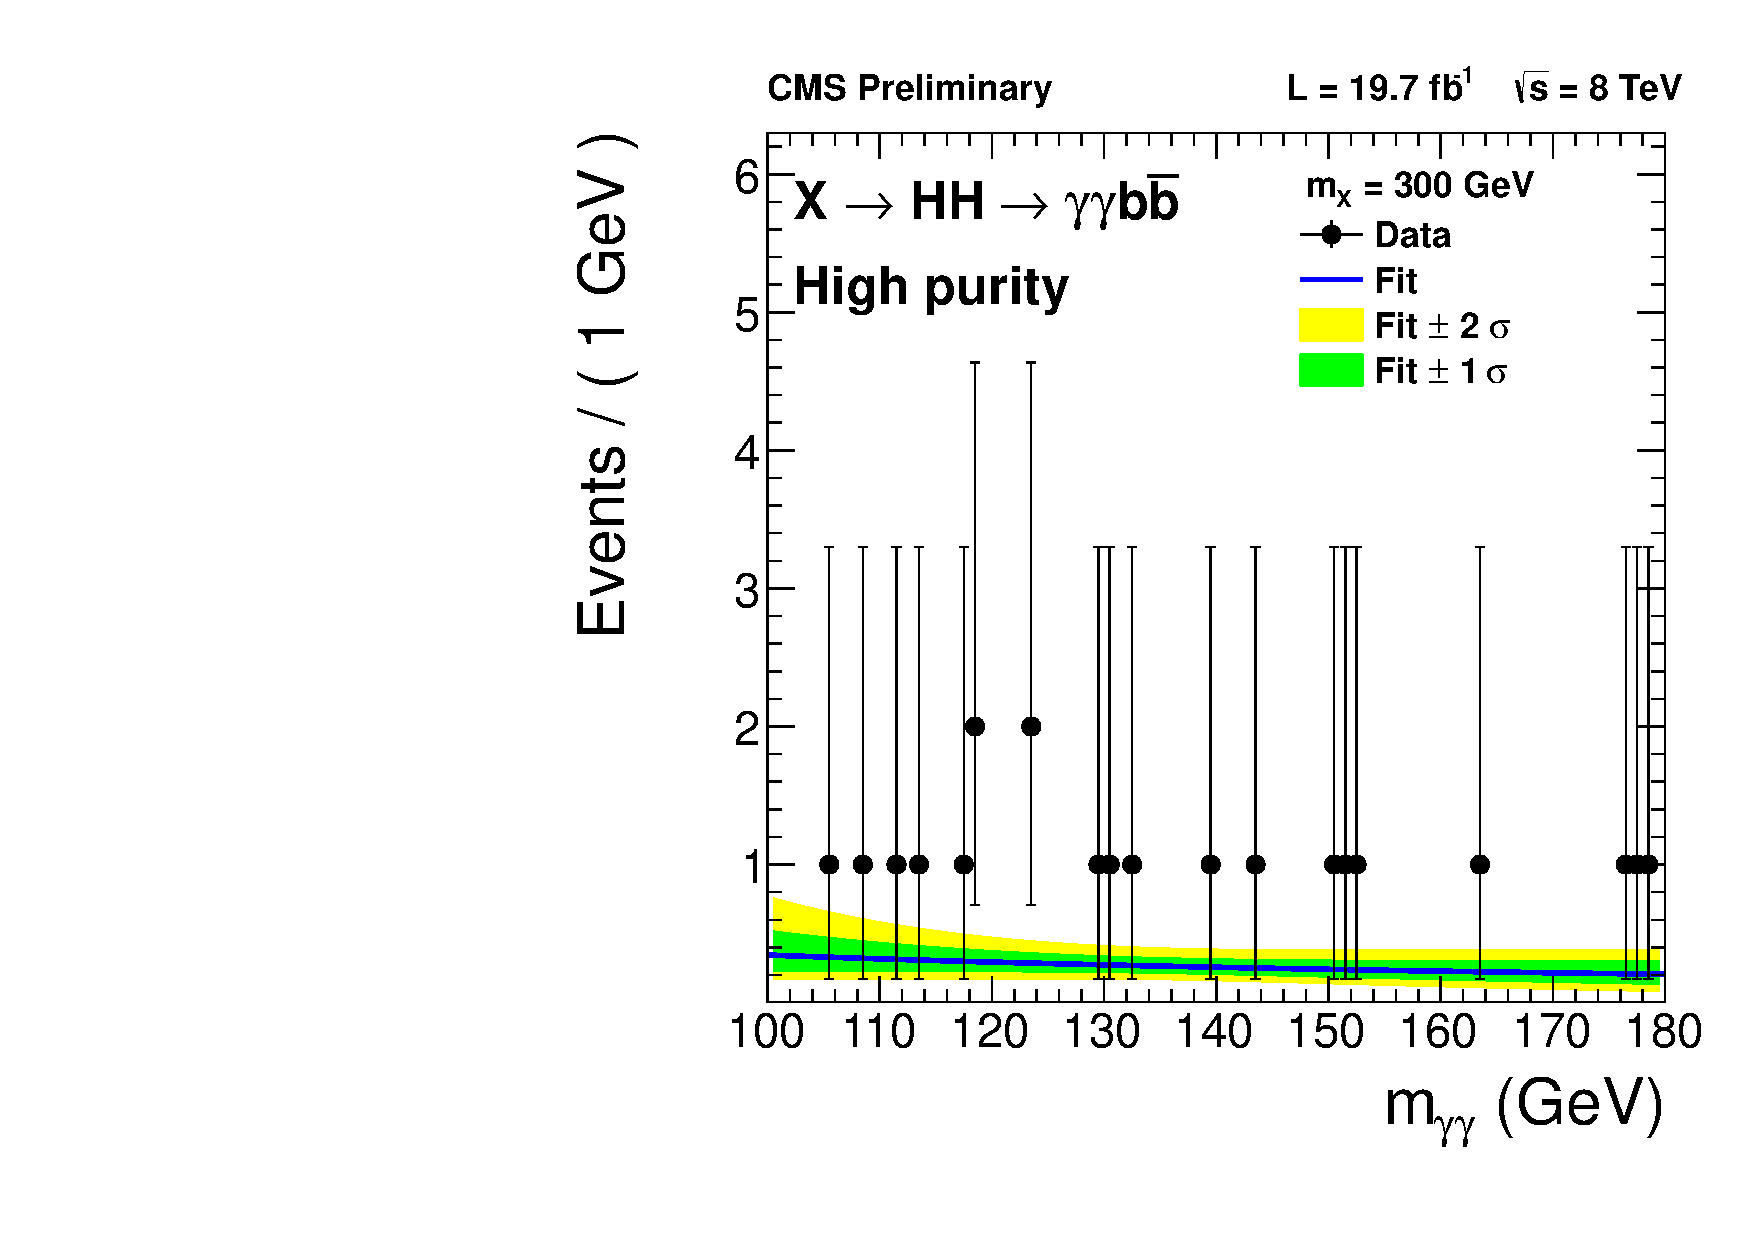
\includegraphics[width=0.45\textwidth]{figures/results/databkgoversig_cat0_300GeV.pdf}
   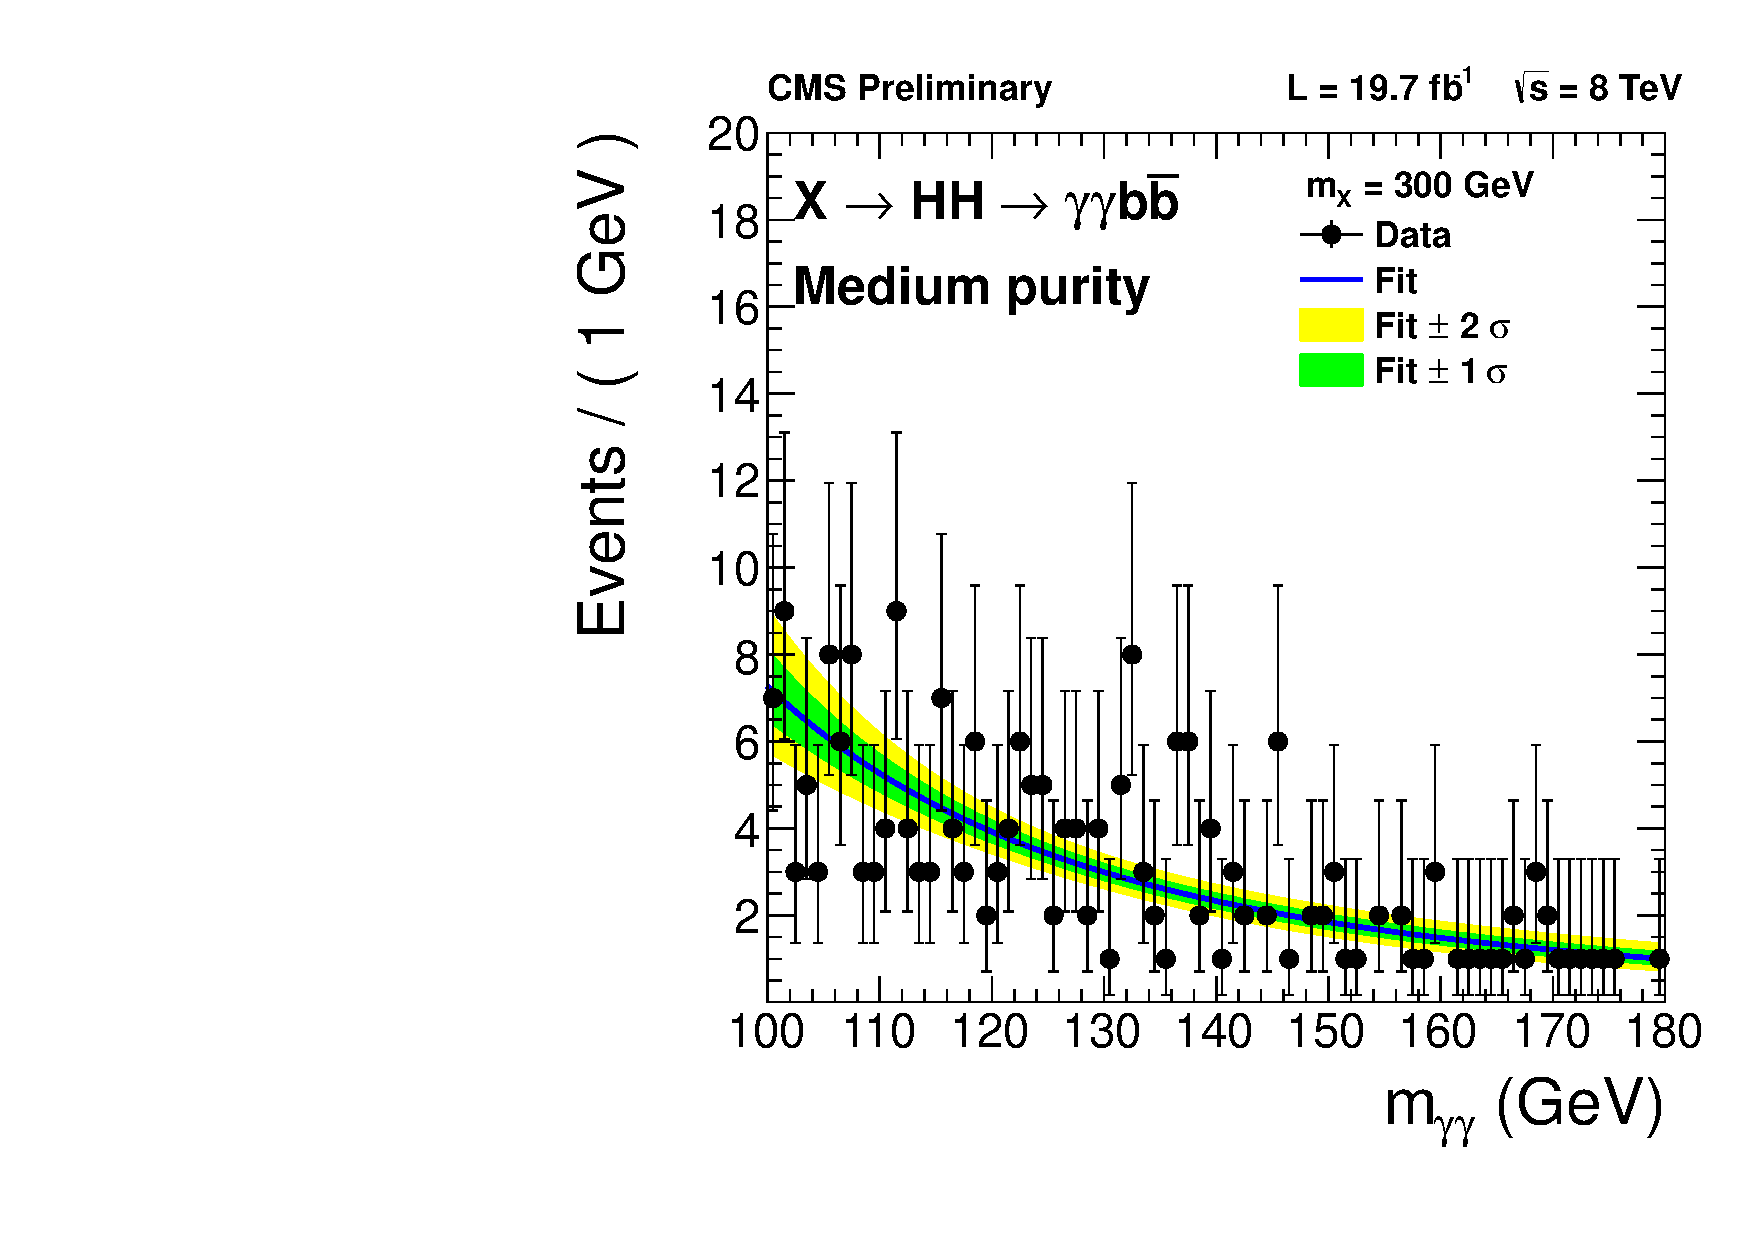
\includegraphics[width=0.45\textwidth]{figures/results/databkgoversig_cat1_300GeV.pdf}
   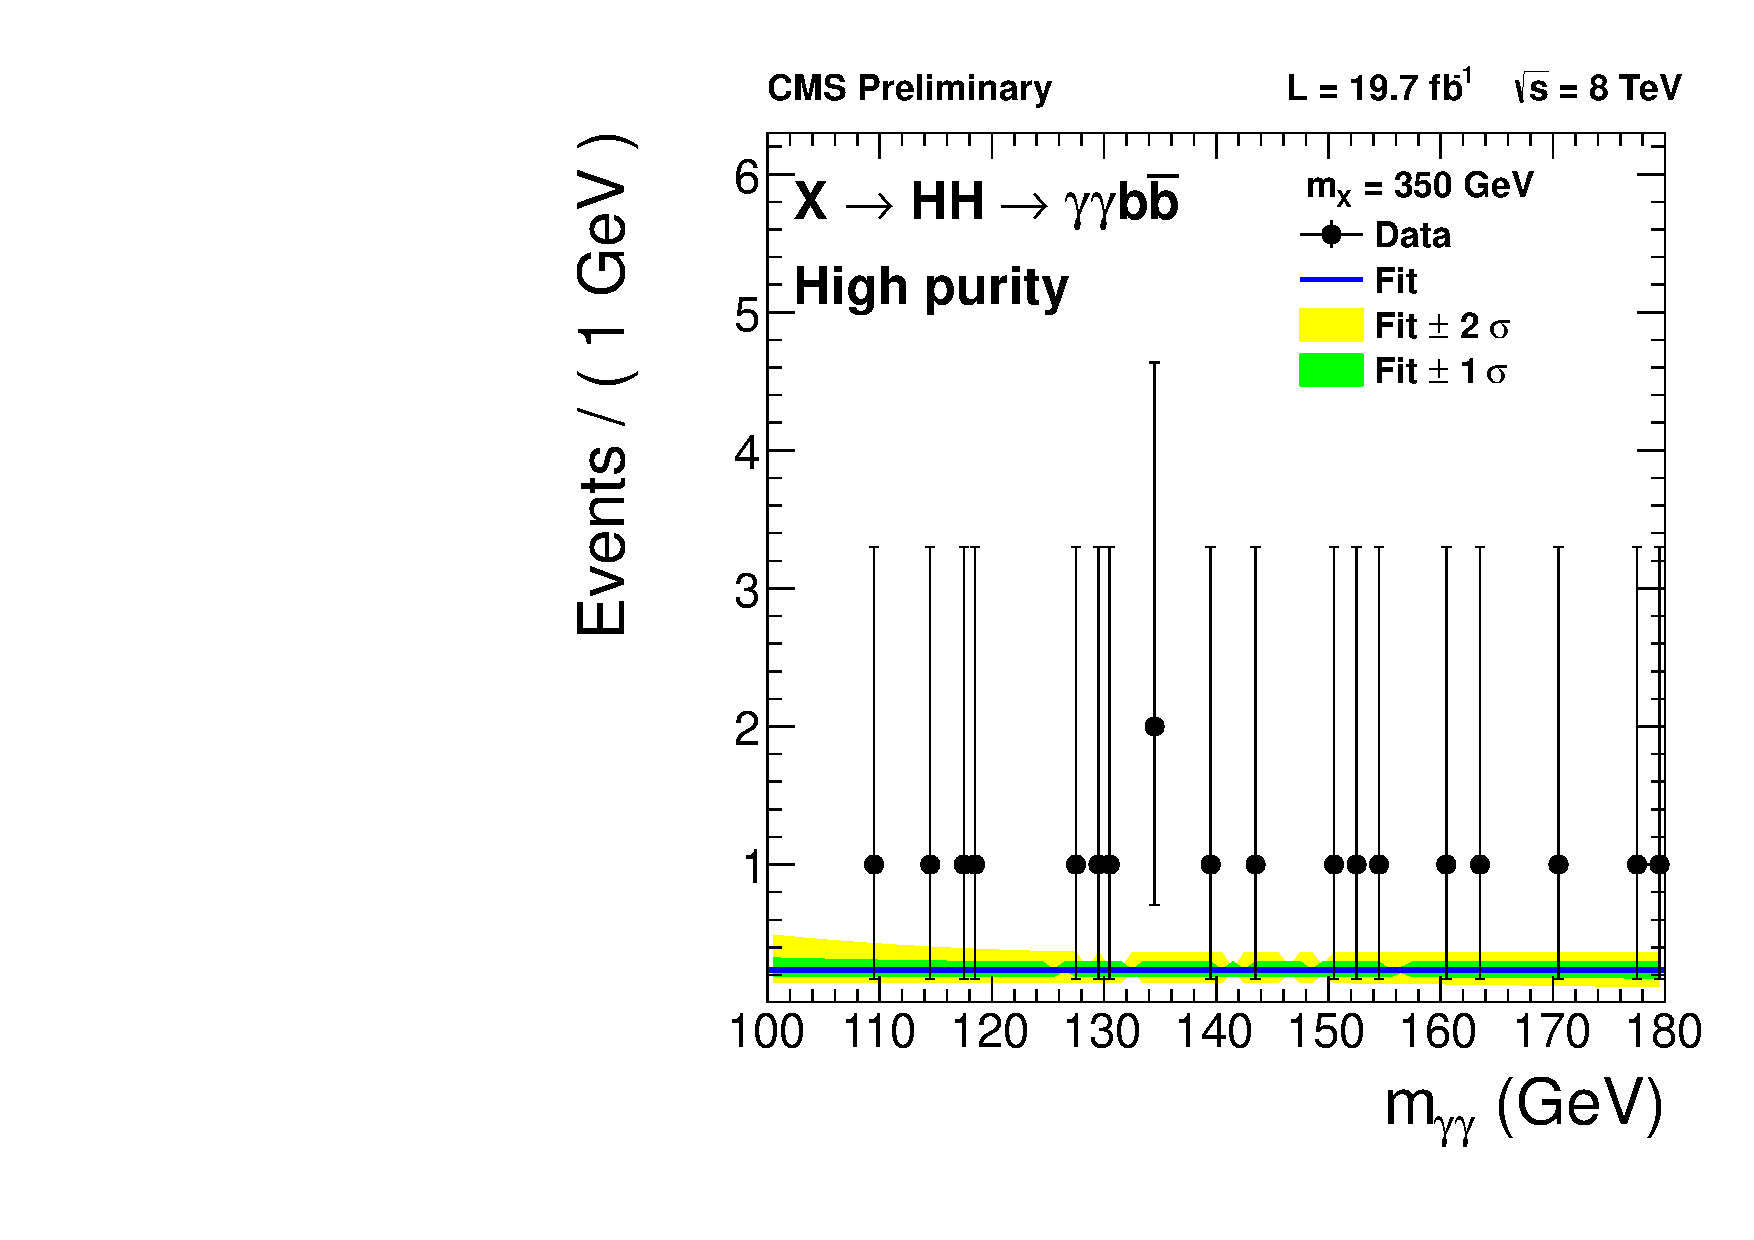
\includegraphics[width=0.45\textwidth]{figures/results/databkgoversig_cat0_350GeV.pdf}
   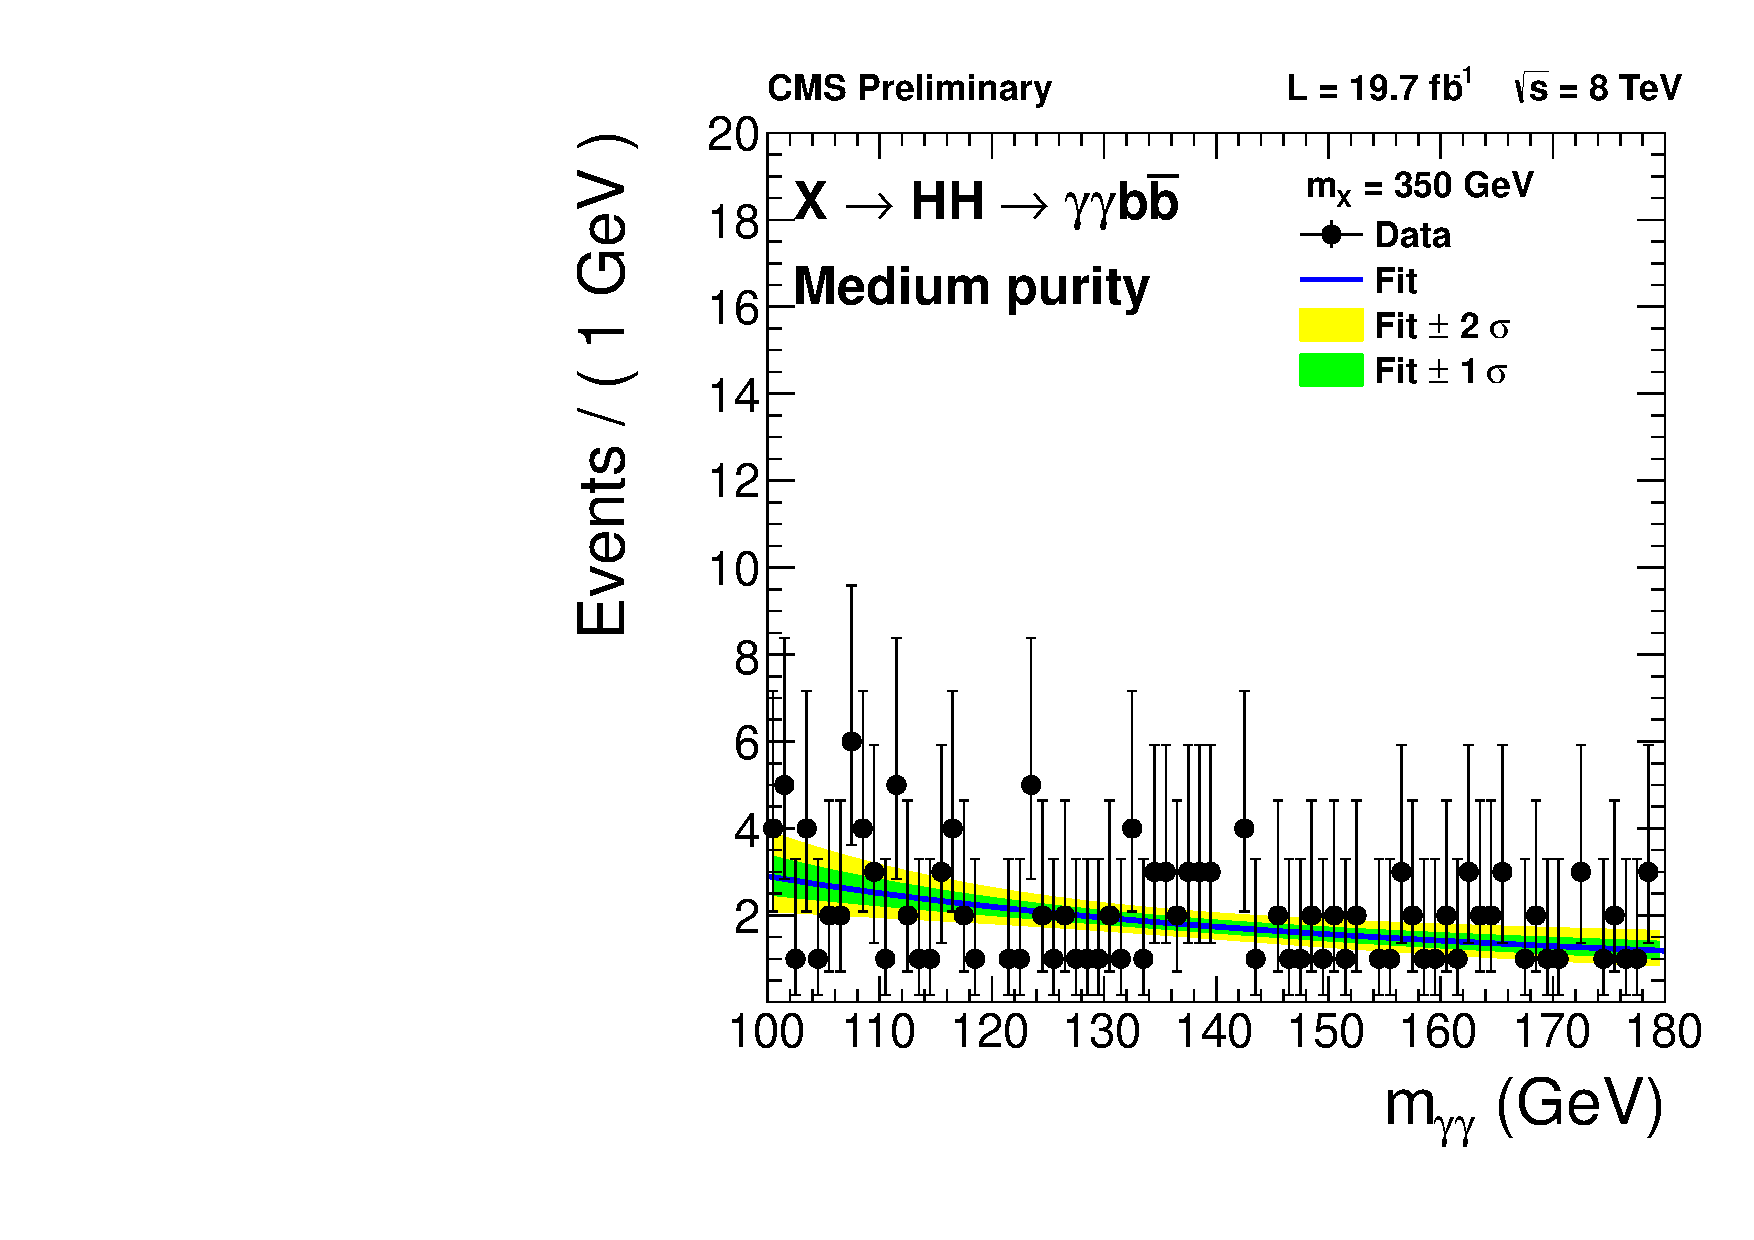
\includegraphics[width=0.45\textwidth]{figures/results/databkgoversig_cat1_350GeV.pdf}
 \end{center}
\caption{Events in the $\Mgg$ spectrum in the high-purity (left column) and medium-purity
(right column) categories for the resonance mass hypotheses 300 GeV (top row) and 350 GeV (bottom row)
The nonresonant component of the background fit is shown in blue
with its corresponding 1$\sigma$ and 2$\sigma$ confidence intervals.}
\label{fig:datafit_300}
\end{figure}

The background fit estimates only the nonresonant contribution arising from diphoton
production. The contribution from SM Higgs production with $\Hgg$ creates a resonance in the
spectrum that mimics the signal process. Each resonant background
contribution is fit to simulation in the same way as the signal,
and the normalization of each contribution fixed to its expected yield, which are summarized
in Table~\ref{table:yield_higgs_lowmass}.
The expected yield for each contribution is small, and the
effect on the expected sensitivity is found to be at most 2\% for all low-mass resonant hypotheses.

\begin{table}[htbp!]
  \centering
  \renewcommand{\arraystretch}{1.4}
  \caption{Expected yields for the resonant backgrounds of the low-mass resonant search at 300 GeV.}
  \begin{tabular}{|c|c|c|}
\hline
Sample & High purity & Medium purity\\
\hline
ggF $\Hgg$                &  0.02  &  0.19 \\
VBF $\Hgg$                &$<$~0.01&  0.04 \\
$WH(\gamma\gamma)$        &$<$~0.01&  0.05 \\
$ZH(\gamma\gamma)$        &$<$~0.01&  0.03 \\
$t\bar{t}H(\gamma\gamma)$ &  0.10  &  0.15 \\
\hline
\end{tabular}

  \label{table:yield_higgs_lowmass}
\end{table}

\subsection{High-mass Resonant Fits}

For the high-mass resonant search, the signal yield is extracted by fitting the $\Mggjjk$ spectrum
in a procedure similar to the one for the low-mass resonant search. The signal model is built
for each mass hypothesis by fitting the $\Mggjjk$ peak in the simulation sample separately for the
two categories. The functional form used is the sum of a Crystal Ball and a Gaussian, with each
constrained to have the same mean. The position of the peak follows the corresponding $m_X$
hypothesis closely,
and the resolution in the peak improves as $m_X$ increases. Figure~\ref{fig:sigfit_500_1000}
shows examples of the signal fit for mass hypotheses of 500 GeV and 1 TeV.

\begin{figure}[htbp!]
 \begin{center}
   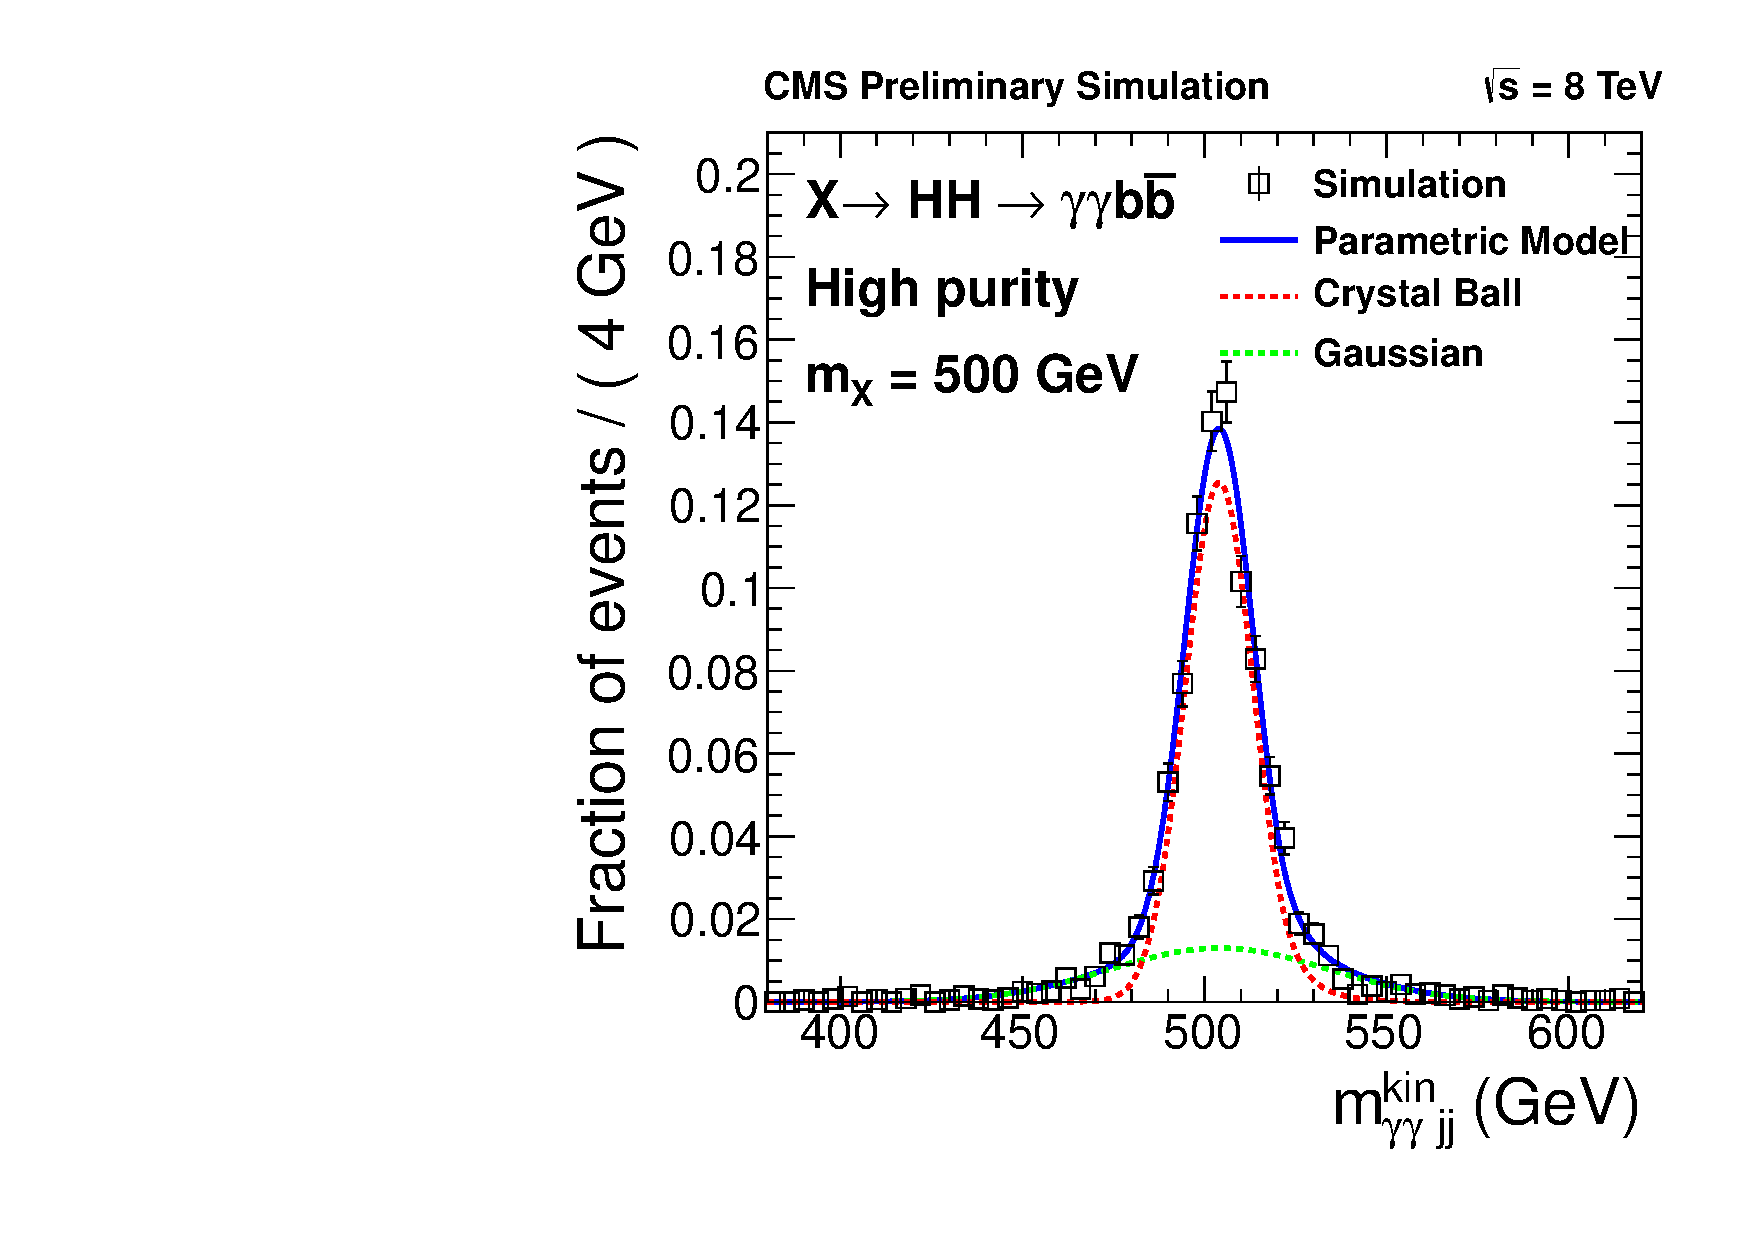
\includegraphics[width=0.45\textwidth]{figures/results/sigmodel_cat0_500GeV.pdf}
   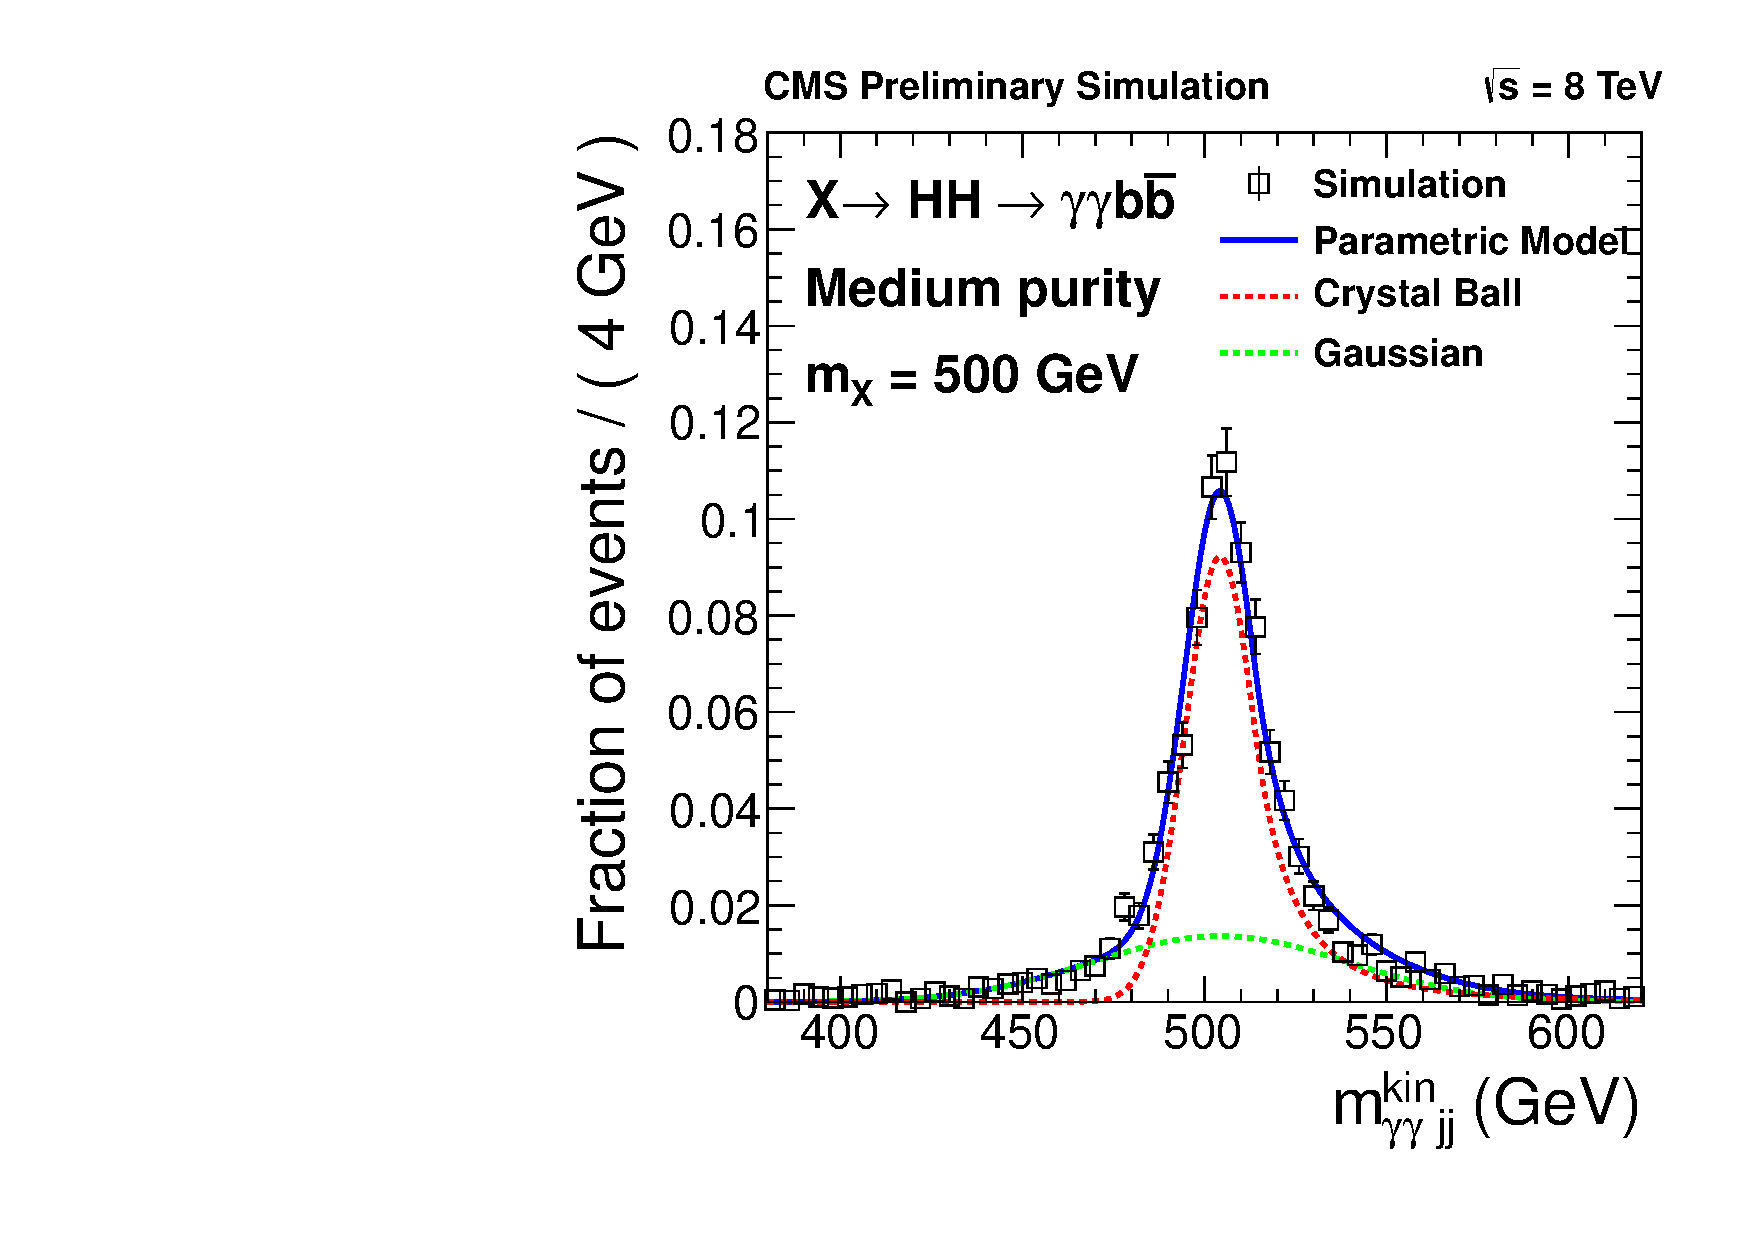
\includegraphics[width=0.45\textwidth]{figures/results/sigmodel_cat1_500GeV.pdf}
   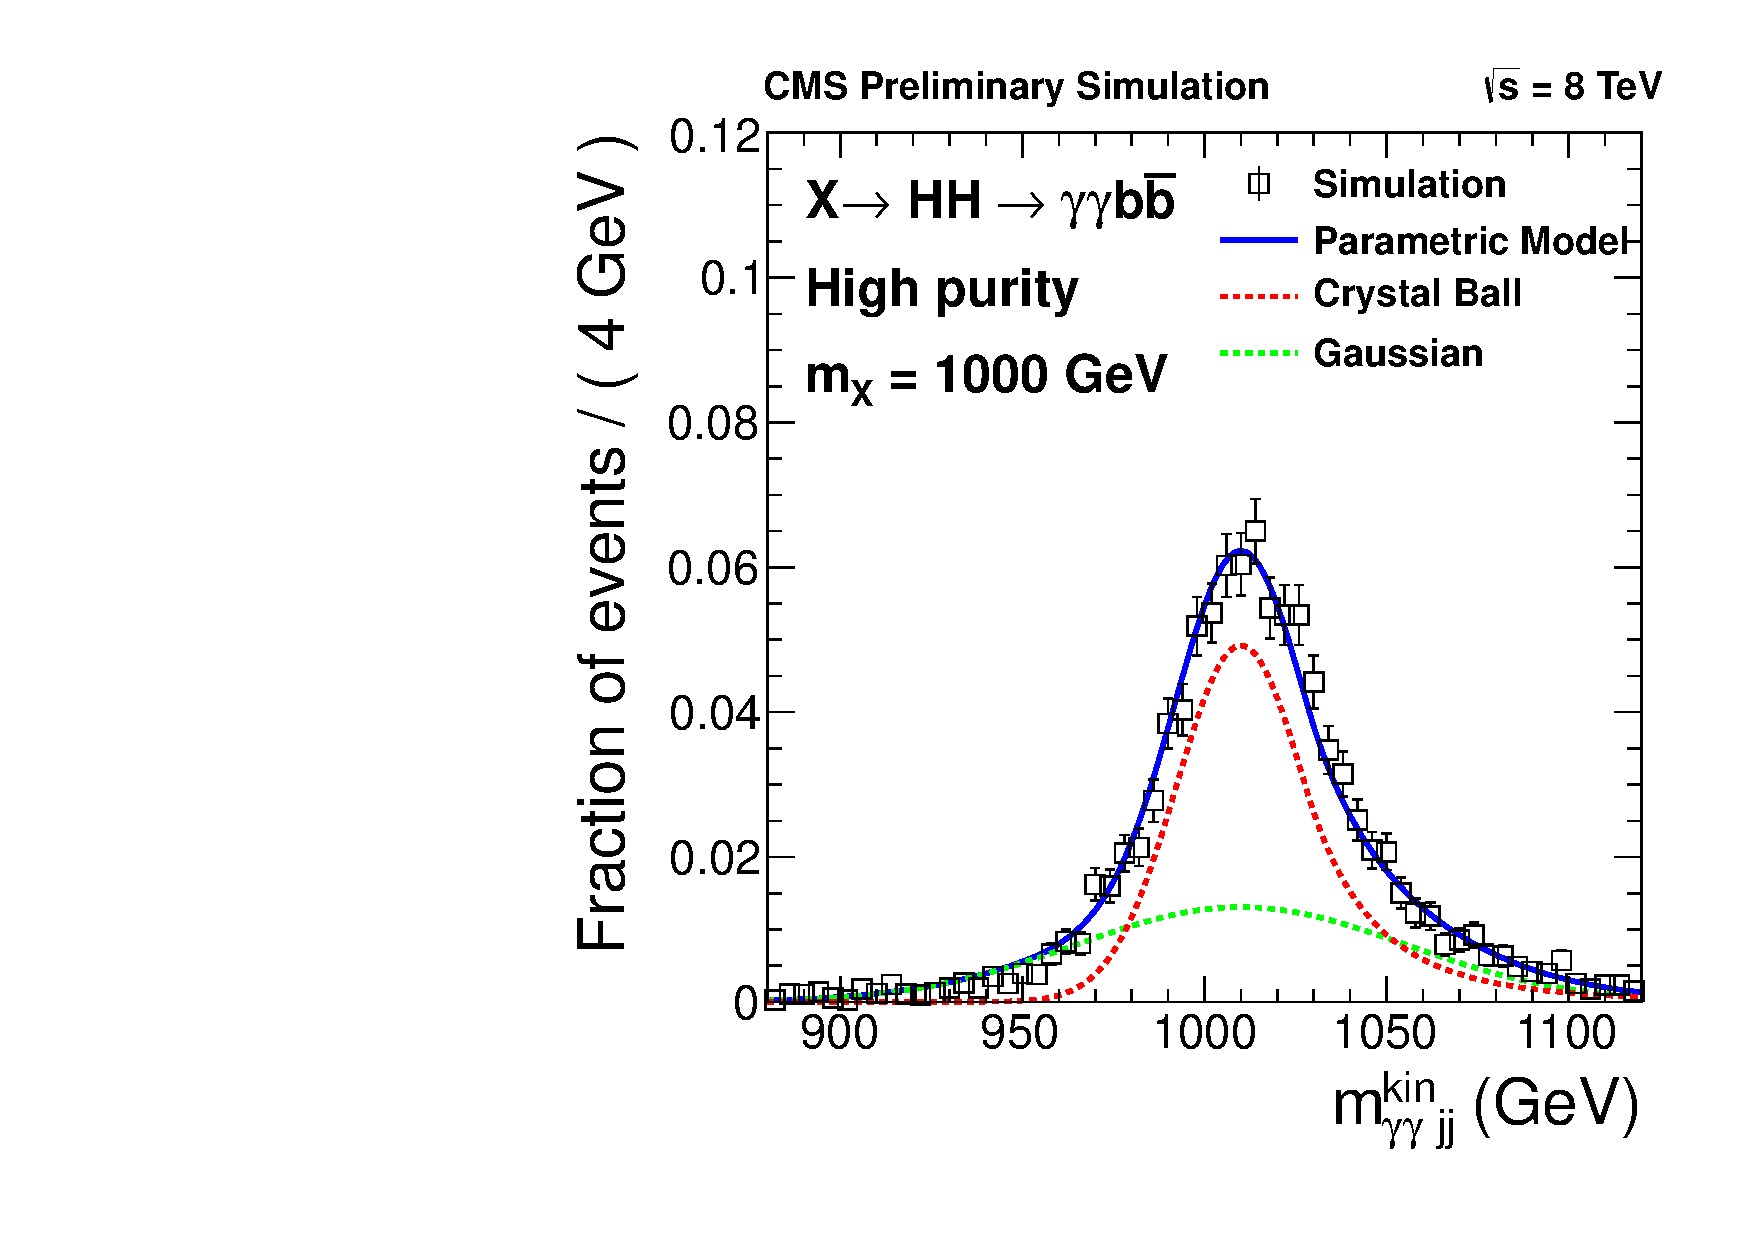
\includegraphics[width=0.45\textwidth]{figures/results/sigmodel_cat0_1000GeV.pdf}
   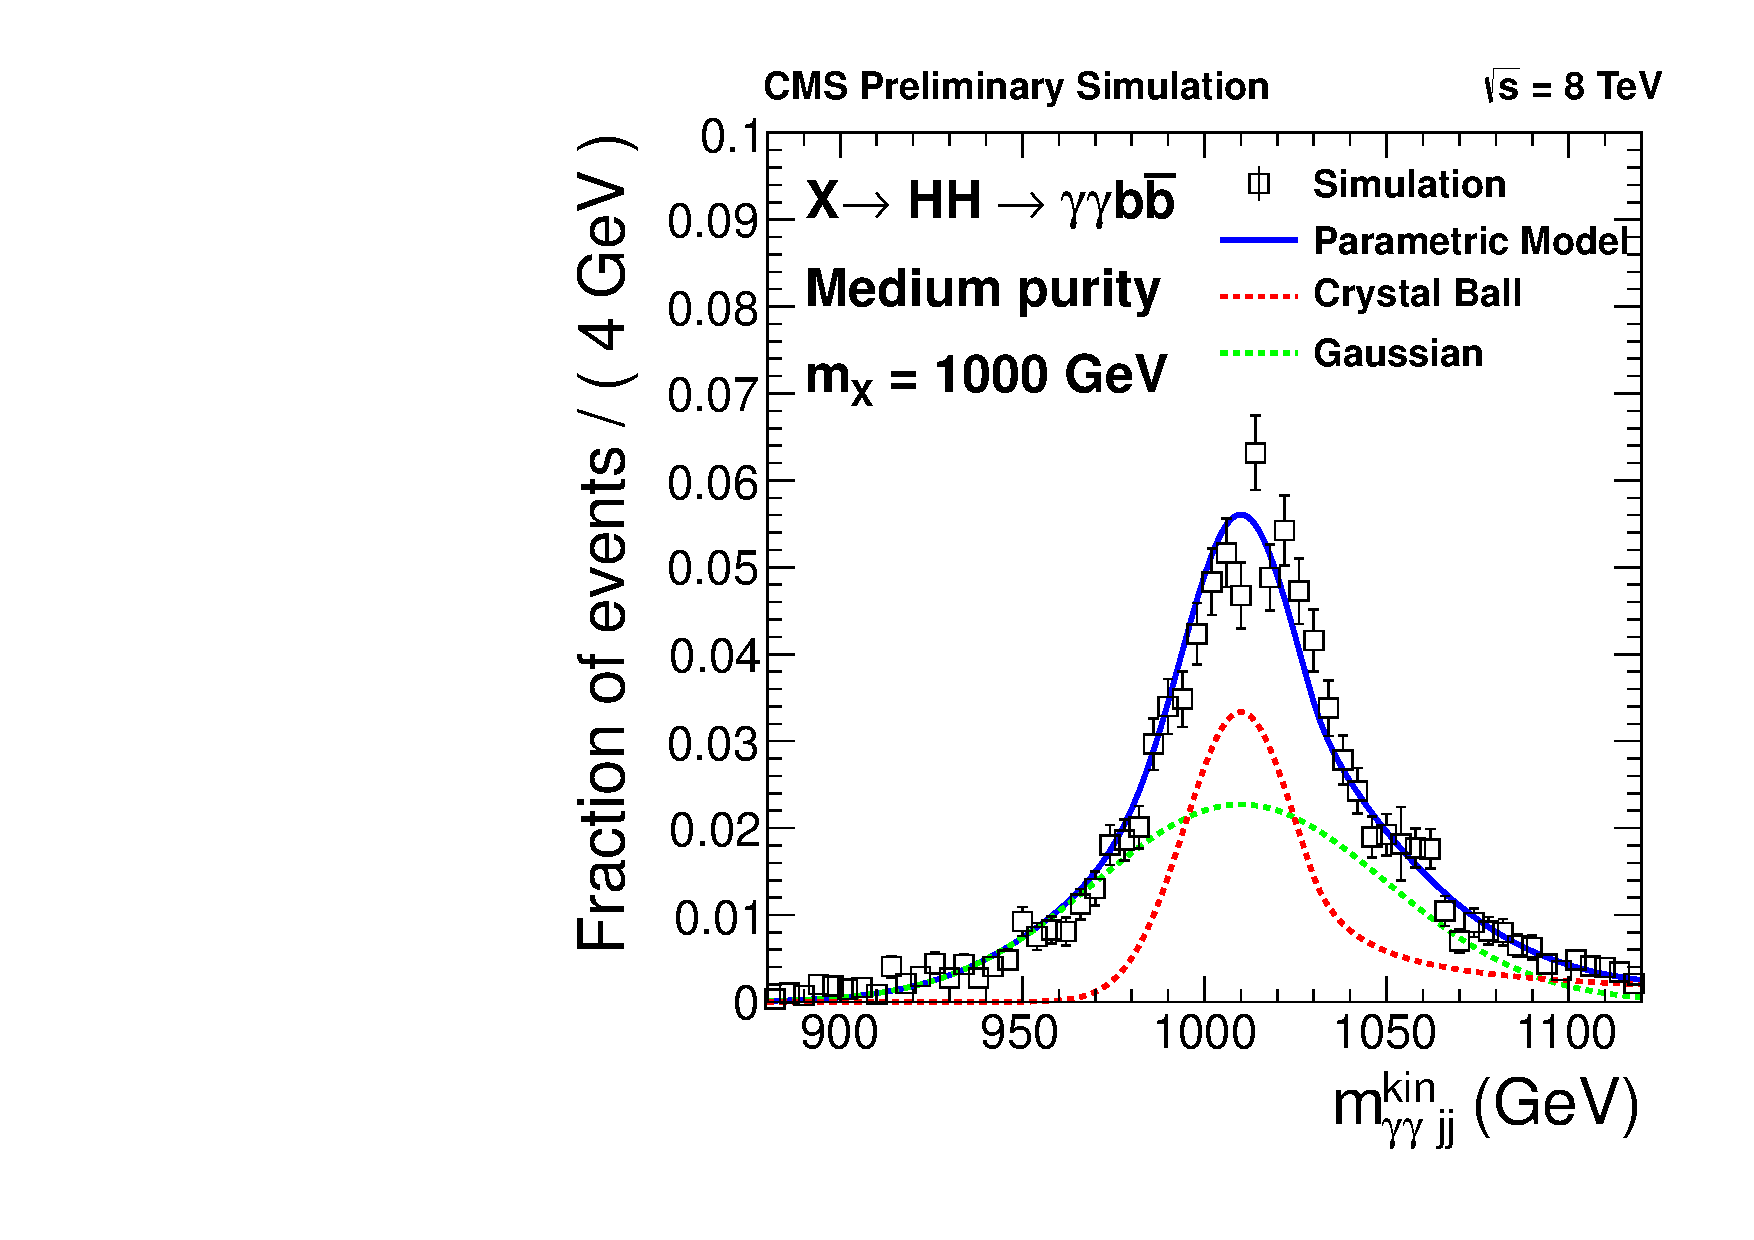
\includegraphics[width=0.45\textwidth]{figures/results/sigmodel_cat1_1000GeV.pdf}
 \end{center}
\caption{Simulated signal shape in the $\Mggjjk$ spectrum for the high-purity (left column)
and medium-purity (right column) categories for the Radion with mass 500 GeV (top row) and
1 TeV (bottom row). The open squares and corresponding
statistical uncertainties represent the simulation.
The blue line represents the signal model fitted to the simulation, while the green dashed line
and the red dashed line represent the two components of the signal model.}
\label{fig:sigfit_500_1000}
\end{figure}


The background estimation is done by fitting the same distribution in each category on the interval
$[320, 1200]$~GeV. The lower edge is chosen to avoid the kinematic turn-on of the background
while ensuring full containment of the 400 GeV signal. The same bias estimation procedure
described for the low-mass resonant search is applied here. The chosen background function is a power
law for both categories, shown in Figure~\ref{fig:datafit_4body}. Note that in this regime,
the SM Higgs background does not have a resonance on the $\Mggjjk$ spectrum, so
there is no resonant contamination from the background.

\begin{figure}[htbp!]
 \begin{center}
   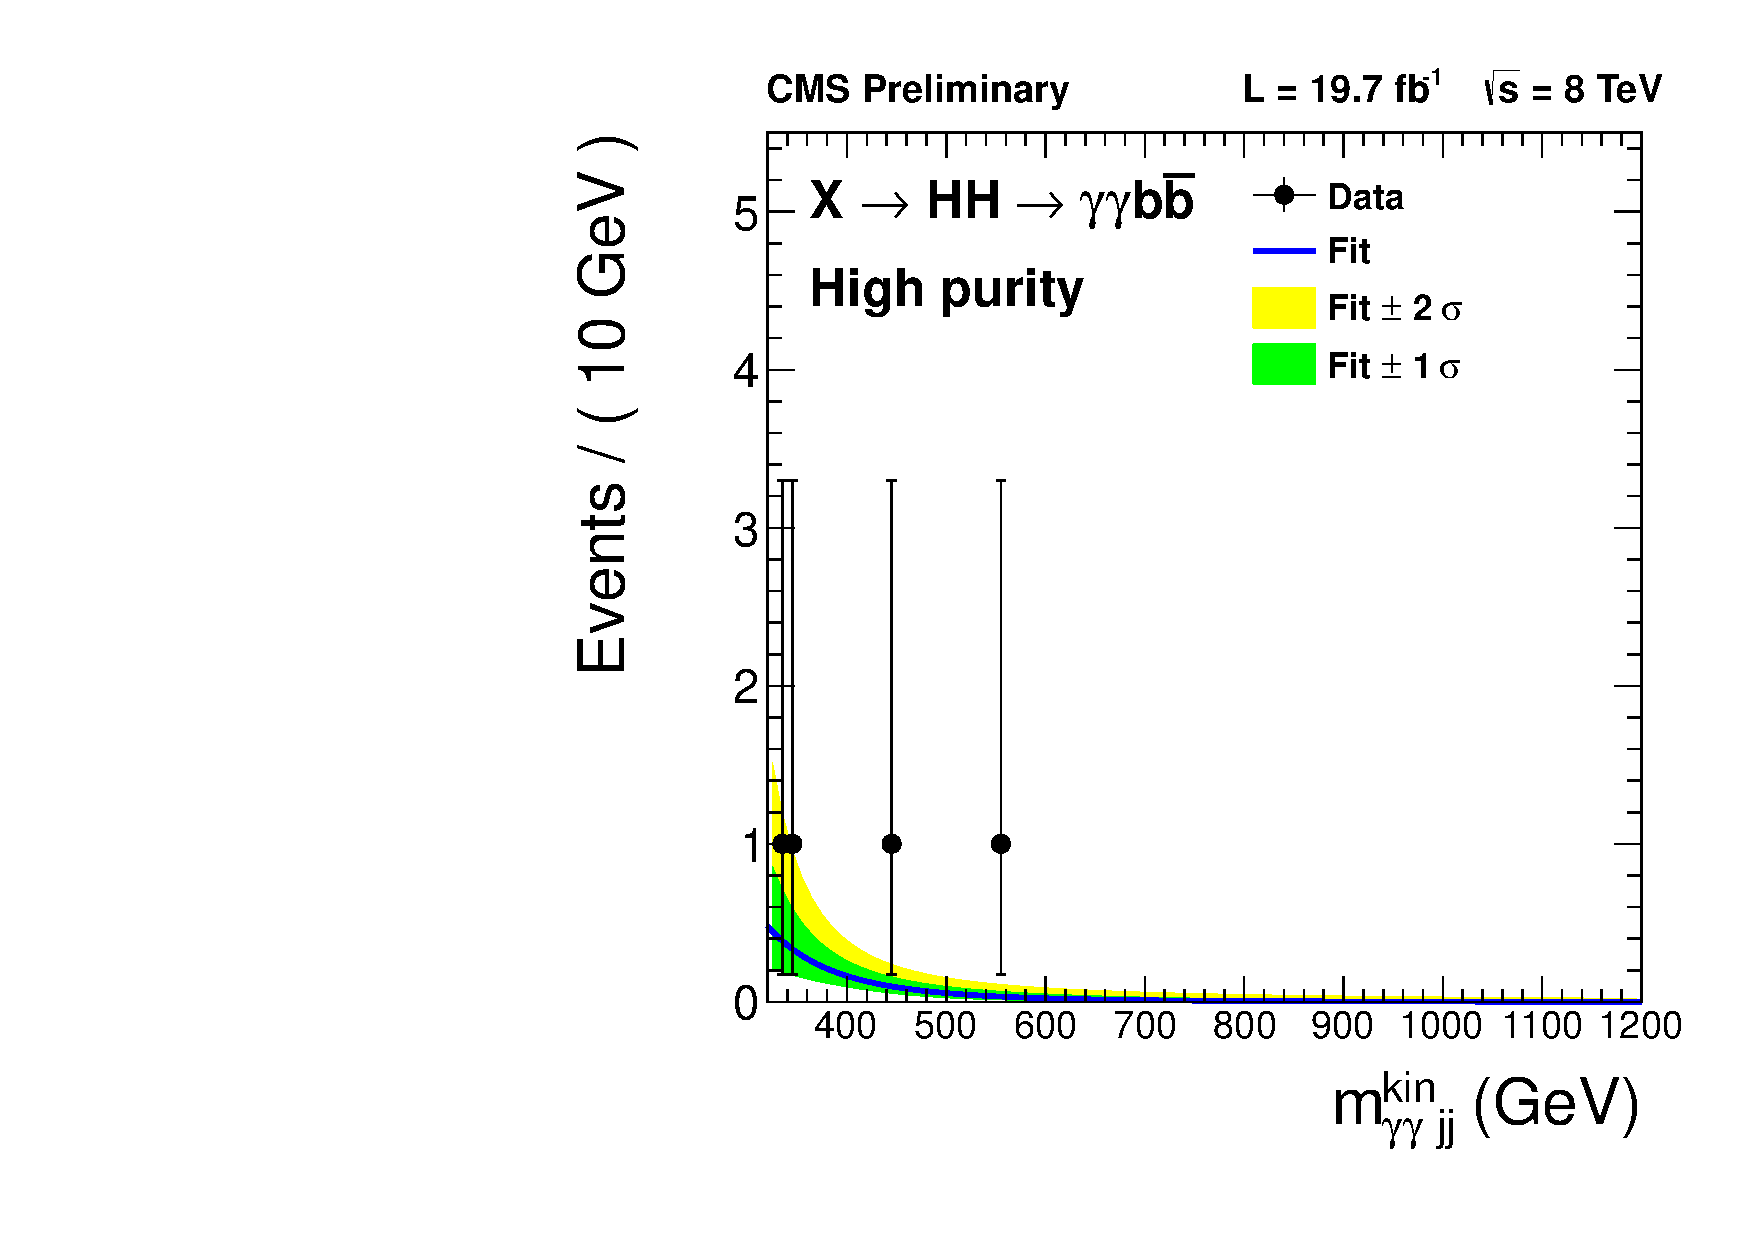
\includegraphics[width=0.45\textwidth]{figures/results/databkgoversig_cat0_4body.pdf}
   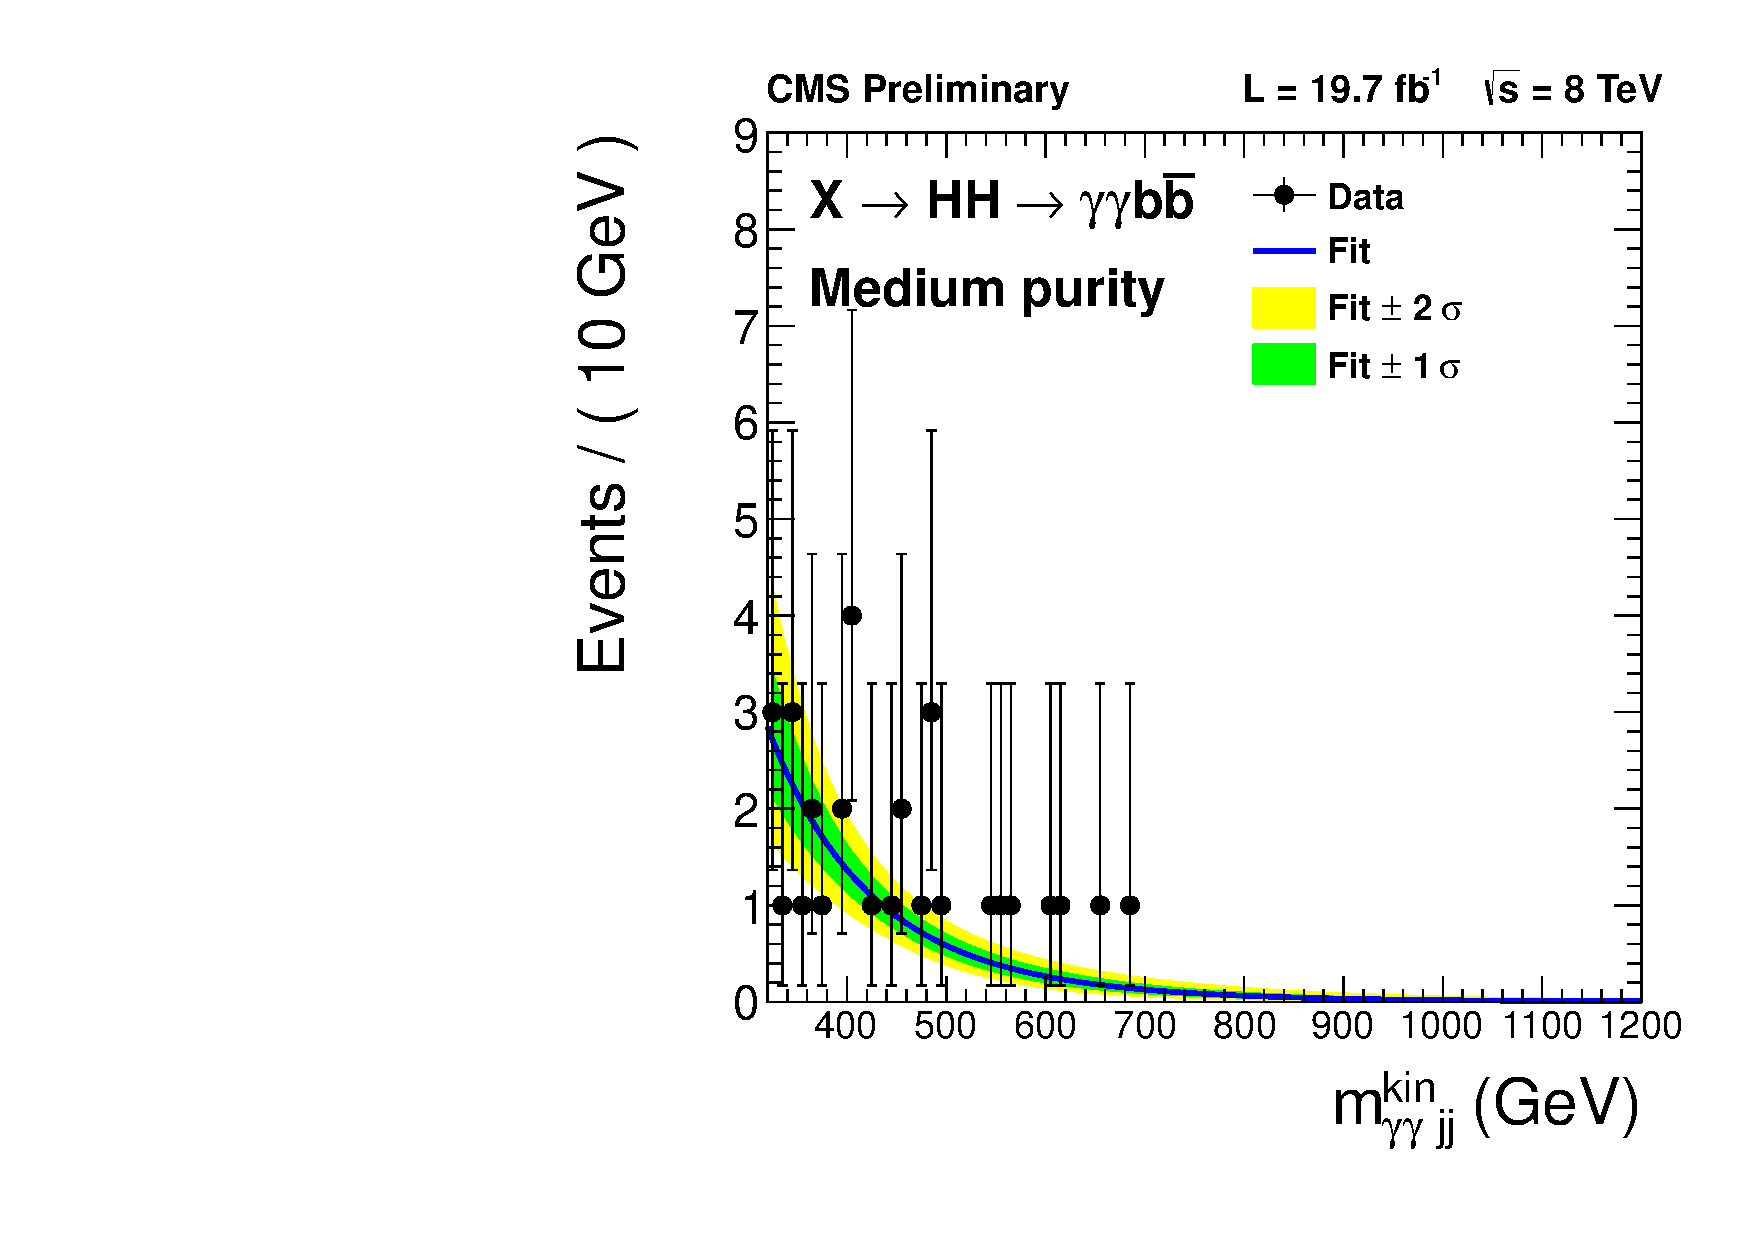
\includegraphics[width=0.45\textwidth]{figures/results/databkgoversig_cat1_4body.pdf}
 \end{center}
\caption{Events in the $\Mggjjk$ spectrum in the high-purity (left) and medium-purity (right)
categories. The background fit is shown in blue
with its corresponding 1$\sigma$ and 2$\sigma$ confidence intervals.}
\label{fig:datafit_4body}
\end{figure}

\section{Nonresonant Fits\label{sec:nonresfits}}

For the SM nonresonant search, the signal yield is extracted by fitting the
$\Mgg \times \Mjj$ plane. The signal model is built by simultaneously fitting both dimensions
for each of the four categories separately.
The functional form used in both dimensions is the sum of a Crystal Ball and
a Gaussian, with each constrained to have the same mean. The background estimation is done by fitting
the same plane in each category on the interval $[100, 180]$~GeV for $\Mgg$ and $[60, 180]$~GeV
for $\Mjj$. The same bias estimation procedure
described for the low-mass resonant search is applied here. The chosen background function is a power
law for both dimensions in all four categories. The SM Higgs production is treated as a resonant
background, and each contribution is fit in the same way as signal with the normalization
of each contribution fixed to the expected yield, given in Table~\ref{table:yield_data_nonres}.

